\documentclass[a4paper]{article}
\usepackage{graphicx} % Required for inserting images
\usepackage{authblk} % For organizing author and affiliation information
\usepackage[czech]{babel} % základní podpora pro češtinu, mj. správné dělení slov
\usepackage[utf8]{inputenc} % vstupní kódování je UTF-8
\usepackage{anyfontsize}
\usepackage{enumitem}
\usepackage{blindtext}
\usepackage{acronym}
\usepackage[left=3cm,right=3cm,bottom=3.5cm]{geometry}
\usepackage{tikz}
\usepackage{multicol}
\usepackage{wrapfig}
\usepackage{caption}
\usepackage{pdfpages}
\usepackage{fancyhdr} % For custom headers and footers
\usepackage{graphicx}
\usepackage{hyperref}

% uvozovky
\newcommand\uvoz[1]{\quotedblbase #1\textquotedblleft}%

% Environment for importing the about_us_page
\newenvironment{importedcontent}{%
  \begingroup
  \renewcommand{\thepage}{\arabic{page}} % Reset page numbering to main document's style
  \pagestyle{empty} % Disable page style for the imported content
  \setcounter{section}{0} % Reset sectioning if desired
}{\endgroup}

% pagestyle
\pagestyle{fancy}
\fancyhf{} % Clear default header and footer
% Header with section and subsection
\fancyhead[R]{\small\textcolor{gray}{\nouppercase{\leftmark}}} % Section name
%\fancyhead[R]{\small\textcolor{gray}{\nouppercase{\rightmark}}} % Subsection name

% Footer with a picture, author name, and some text
\fancyfoot[L]{\raisebox{-13pt}{
\includegraphics[width=2.5cm]{pics/FEKT_zkratka_logo_RGB_CZ.png}}}
\fancyfoot[C]{\thepage}
\fancyfoot[R]{\small\textcolor{gray}{Inteligentní hangár\\Dokumentace}} % Add your desired text
\renewcommand{\headrulewidth}{0pt}

\begin{document}

\begin{titlepage}
    \begin{center}
        \vspace*{1cm}
            
        \Huge
        \textbf{Inteligentní hangár}\\
        \Large
        \textbf{Dokumentace}
            
        \vspace{0.5cm}
        \LARGE
            
        \vspace{1.5cm}
            
        \textbf{Emanuel Antol,}
        \textbf{Hugo Bohácsek,}\\
        \textbf{Lukáš Lenčeš,}
        \textbf{Lukáš Lev,}\\
        \textbf{Tomáš Proks,}
        \textbf{Martin Strouhal}
            
        \vfill
            
        FEKTTeams\\
        2024
            
        \vspace{0.8cm}
            
        
\includegraphics[width=0.4\textwidth]{pics/FEKT_zkratka_logo_RGB_CZ (1).png}
            
        \Large
        FEKT, VUT\\
        \today
        %28. 11. 2024
    \end{center}
\end{titlepage}
\newpage

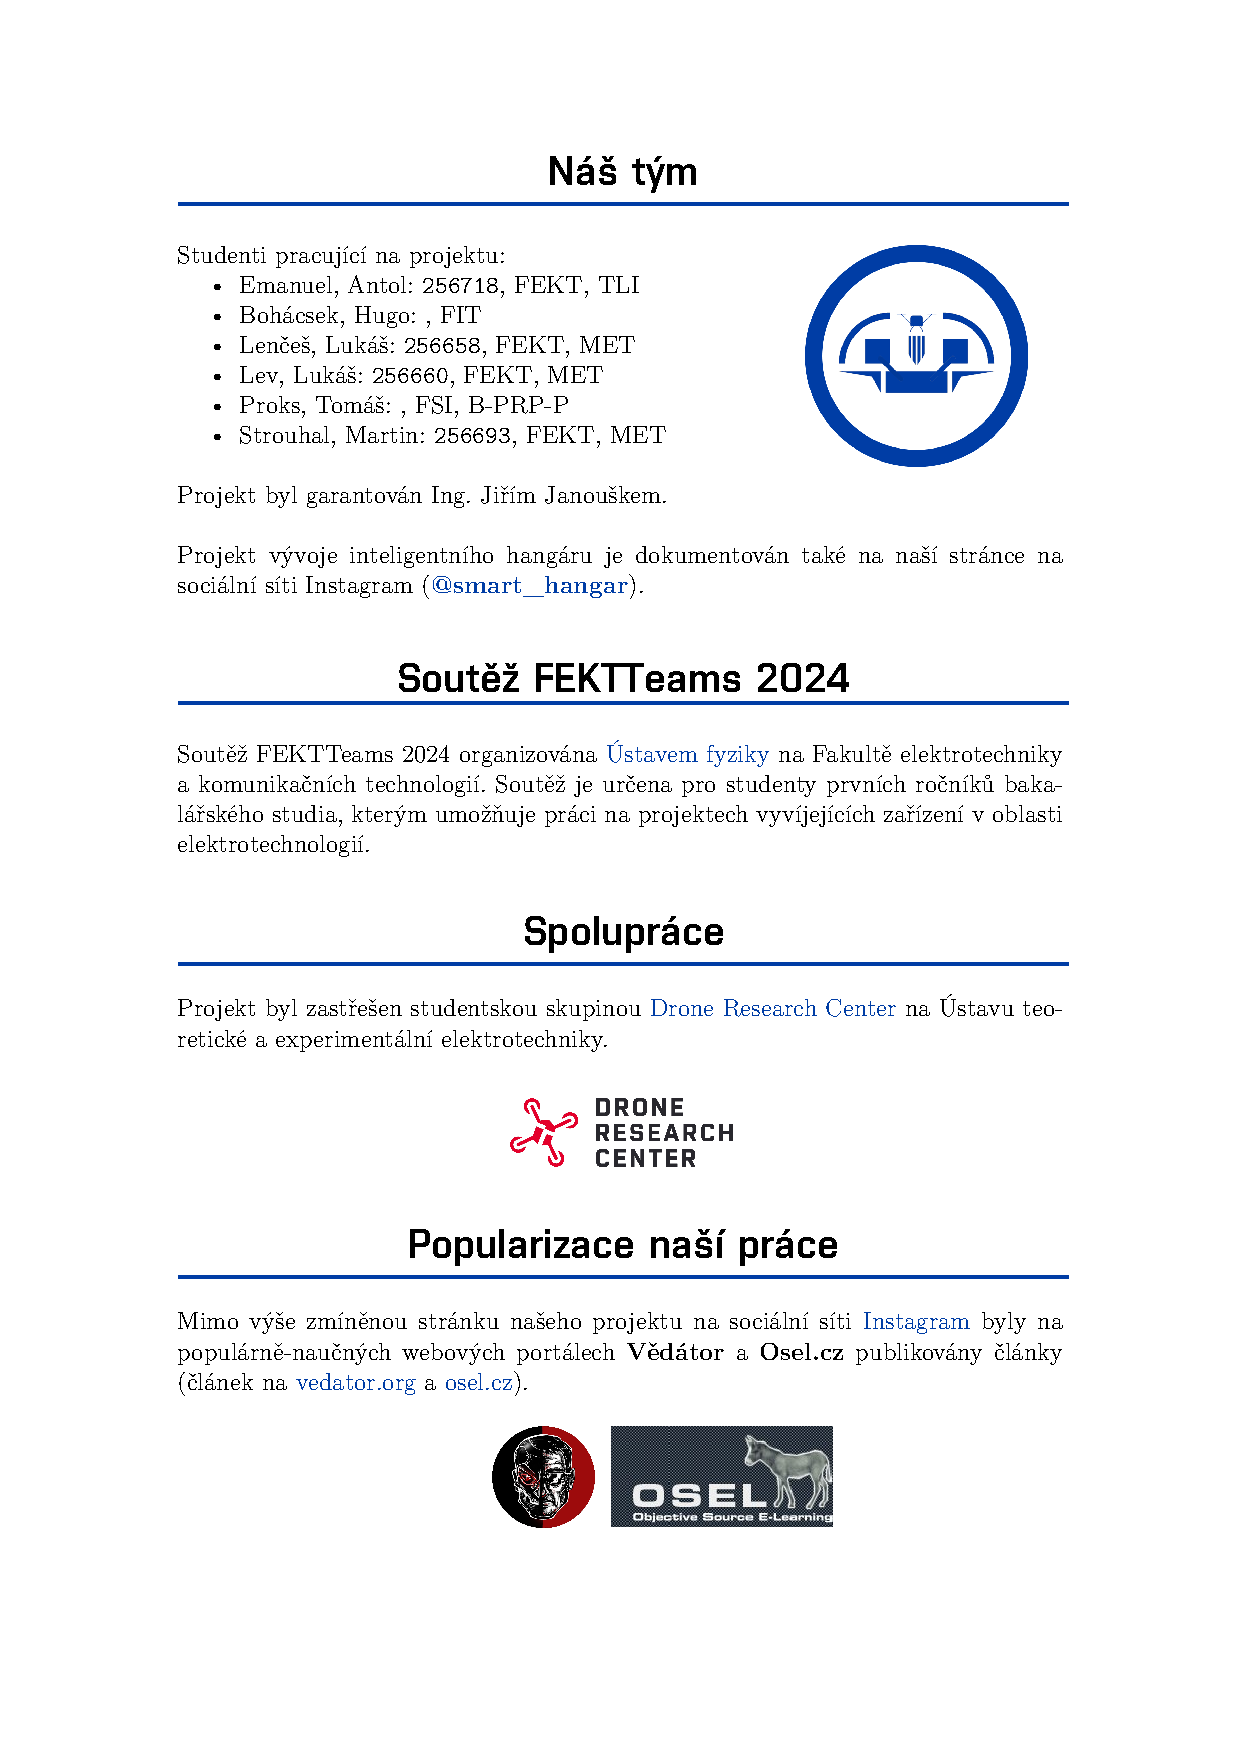
\includepdf{about_us_page/about_us_page.pdf}
%\begingroup
%    \documentclass{article} % Use article or a minimal class

% Load the necessary packages locally
\usepackage{tikz}
\usepackage{hyperref}
\usepackage{xcolor}
\usepackage{graphicx}
\begin{document}
	\pagestyle{empty}
    
	%\vspace{2cm} % odsazeni po nadpisu
	%\begin{multicols*}{2}  % the * with the multicols make them not to be equalized
		\selectfont
            %\fontsize{10}{10}
            %\selectfont
		\section{Náš tým}
                Studenti pracující na projektu:
                \begin{itemize}
                    \item Emanuel, Antol: \texttt{256718}, FEKT, TLI
                    \item Bohácsek, Hugo: \texttt{}, FIT
                    \item Lenčeš, Lukáš: \texttt{256658}, FEKT, MET
                    \item Lev, Lukáš: \texttt{256660}, FEKT, MET
                    \item Proks, Tomáš: \texttt{}, FSI, B-PRP-P
                    \item Strouhal, Martin: \texttt{256693}, FEKT, MET
                \end{itemize}
                
                \vspace{.5cm}
                \noindent
                Projekt byl garantován Ing. Jiřím Janouškem.\\
                \begin{tikzpicture}[remember picture, overlay]
                    \node[anchor=north west, xshift=13.5cm, yshift=-4cm] at (current page.north west) {
                        
\includegraphics[width=0.25\textwidth]{about_us_page/smart_hangar.png}
                    };
                \end{tikzpicture}

                \noindent
                Projekt vývoje inteligentního hangáru je dokumentován také na naší stránce na sociální síti Instagram (\href{https://www.instagram.com/smart_hangar/}{\textbf{@smart\_hangar}}).
                               
            \section{Soutěž FEKTTeams 2024}
                Soutěž FEKTTeams 2024 organizována \href{https://www.ufyz.fekt.vut.cz/}{Ústavem fyziky} na Fakultě elektrotechniky a komunikačních technologií. Soutěž je určena pro studenty prvních ročníků bakalářského studia, kterým umožňuje práci na projektech vyvíjejících zařízení v oblasti elektrotechnologií.
                %\begin{wrapfigure}{r}{0.25\textwidth}
                %    
\includegraphics[width=0.9\linewidth]{about_us_page/logo_ufyz.png} 
                %\end{wrapfigure}
            \section{Spolupráce}    
                Projekt byl zastřešen studentskou skupinou \href{https://www.utee.fekt.vut.cz/drone-research-center}{Drone Research Center} na Ústavu teoretické a experimentální elektrotechniky.\\
                \vspace{1.5cm}
                \begin{tikzpicture}[remember picture, overlay]
                    \node[anchor=north west, xshift=\textwidth/2+1cm, yshift=-18.45cm] at (current page.north west) {
                        
\includegraphics[width=0.25\textwidth]{about_us_page/drone_research_center.png}
                    };
                \end{tikzpicture}
            \section{Popularizace naší práce}
                Mimo výše zmíněnou stránku našeho projektu na sociální síti \href{https://www.instagram.com/smart_hangar/}{Instagram} byly na populárně-naučných webových portálech \textbf{Vědátor} a \textbf{Osel.cz} publikovány články (článek na \href{https://vedator.org/2024/08/autonomni-drony-vznikaji-uz-i-v-cesku-jeden-kuti-v-brne/}{vedator.org} a \href{https://www.osel.cz/13580-autonomni-hnizdo-inovativni-hangar-z-vut-prinasi-technologickou-revoluci.html}{osel.cz}).
                \begin{tikzpicture}[remember picture, overlay]
                    \node[anchor=north west, xshift=82mm, yshift=-24cm] at (current page.north west) {
                        
\includegraphics[width=0.115\textwidth]{about_us_page/vedator.png}
                    };
                \end{tikzpicture}
                \begin{tikzpicture}[remember picture, overlay]
                    \node[anchor=north west, xshift=102mm, yshift=-24cm] at (current page.north west) {
                        
\includegraphics[width=0.25\textwidth]{about_us_page/osel.jpg}
                    };
                \end{tikzpicture}
	%\end{multicols*}

\end{document}
%\endgroup

% toc
\tableofcontents

\section{Akronymy}
\begin{acronym}
    \acro{LP}{Landing Pad, přistávací plocha hangáru}    
    \acro{UNO}{Arduino UNO, jednodeskový počítač}
    \acro{RPI}{Raspberry Pi 5, jednodeskový počítač}
\end{acronym}
\newpage

\section{Úvod}
V súčasnom rýchlo sa meniacom technologickom svete sa drony stávajú čoraz bežnejším nástrojom na vykonávanie širokej škály úloh – od monitorovania cez kreatívnu činnosť, až po záchranné operácie či logistiku. S narastajúcim dopytom po ich efektívnom a flexibilnom využití vzniká potreba inovatívnych riešení, ktoré zlepšia ich funkčnosť, údržbu a prevádzkovú pripravenosť. Cieľom tohto projektu je vývoj pokročilej modulárnej dokovacej stanice pre drony, ktorá umožní ich použitie v statických aj prenosných podmienkach, pričom poskytne optimálne prostredie pre dron v čase, keď nie je v prevádzke alebo počas nabíjania.\\

\noindent
Modulárnu dokovaciu stanicu sme chceli navrhnuť tak, aby poskytovala maximálnu flexibilitu a prispôsobila sa rôznym potrebám používateľov. Základným princípom je preto modularita, čo znamená, že dokovacia stanica by mala pozostávať z jednotlivých modulov, pomocou ktorých je možné dokovaciu stanicu jednoducho prispôsobiť na konkrétne použitie. V statickom režime bude stanica schopná fungovať ako pevná jednotka umiestnená napríklad na súkromnom pozemku, kde bude dron slúžiť na monitorovanie a zabezpečenie. Podobne môže byť nasadená aj na verejných priestranstvách, ako sú parky či mestské centrá, kde môže podporovať zdravotnícke a záchranné služby v prípade potreby.\\

\noindent
Pre prenosné použitie by mala dokovacia stanica navrhnutá tak, aby ju bolo možné jednoducho pripojiť k vozidlu, čím sa rozšíria jej možnosti nasadenia, napríklad v rámci mobilných operácií alebo v teréne. Dôležitou funkciou prenosného režimu bude možnosť oddelenia \uvoz{hlavného modulu} (\acs{LP}), ktorý by mal obsahovať všetko potrebné pre nabíjanie drona a komunikáciu s dronom od zvyšku stanice, čo uľahčí prepravu a montáž na rôzne typy vozidiel.\\

\noindent
Jednou z najdôležitejších funkcií dokovacej stanice je udržiavanie optimálneho prostredia pre dron, v čase, kedy nie je v prevádzke. Prostredie, v ktorom je dron uložený, zohráva zásadnú úlohu pri zabezpečení jeho dlhej životnosti a pripravenosti na okamžité použitie. Stanica by preto mala byť vybavená systémom termoregulácie, ktorý zabezpečí udržiavanie vhodnej teploty, čo je dôležité najmä v extrémnych podmienkach. Okrem toho by mala obsahovať aj systém monitorovania vlhkosti, čím by sa malo zabrániť kondenzácii alebo nabíjaniu drona v čase, kedy bolo prítomné veľké množstvo vlhkosti, ktorá by mohla poškodiť elektroniku dronu.\\

\noindent
Stanica, alebo konkrétnejšie \uvoz{vonkajší modul} by mal poskytovať aj fyzickú ochranu dronu pred vonkajšími vplyvmi, ako sú prach, nečistoty, silné poveternostné podmienky či potenciálne mechanické poškodenia. Vďaka tomu bude dron vždy pripravený na nasadenie v čo najkratšom čase.\\

\noindent
Ďalšou dôležitou funkciou každej dokovacej stanice je automatické nabíjanie dronu, ktoré by malo zabezpečiť, že dron bude vždy pripravený na použitie. Nabíjací systém by mal byť integrovaný priamo do stanice, čo eliminuje potrebu manuálneho nabíjania. Stanica by taktiež mala poskytovať aj možnosť monitorovania stavu dronu prostredníctvom senzorov a kamier zabudovaných priamo v stanici. Tieto senzory by mali neustále sledovať vonkajšiu a vnútornú teplotu, vlhkosť, stav batérie dronu a iné kľúčové parametre a umožniť tak vzdialenému operátorovi urobiť si obraz o vonkajších a vnútorných podmienkach.\\

\noindent
V prípade výpadku elektrickej energie by naša dokovacia stanica mala taktiež byť vybavená internou batériou, ktorá zabezpečí nepretržité fungovanie stanice aj dronu počas výpadku prúdu. Táto záložná energia by mala  dronu umožniť pokračovať v práci a naďalej pokračovať v monitorovaní a ochrane dronu, čím sa predíde rizikám, ktoré by mohli nastať v prípade neplánovaného prerušenia elektrického napájania. Modulárny design batérie zase zabezpečí možnosť prispôsobenia kapacity vnútornej batérie podľa porieb konkrétneho nasadenia.\\

\noindent
Všetkými týmito funkciami by sme chceli pripraviť našu dokovaciu stanicu na fungovanie vo veľkom rozsahu vonkajších podmienok a zaistiť jej spoľahlivé dlhodobé fungovanie bez nutnosti vonkajšieho zásahu, aj v nepríjemých krítových situáciách.\\

\noindent
Táto dokumentácia poskytuje detailný pohľad na technické riešenia a komponenty projektu, vrátane návrhu hardvéru a softvéru, použité technológie a podrobné informácie o funkciách a prevádzke stanice.
 

\section{Mechanický design} \label{sec:konstrukce}
    Základní koncept konstrukce hangáru vychází z krychlovitého tvaru s rozevírající se vrchní pohyblivou částí představující dveře a s veškerou elektronikou a výpočetní technikou umístěnou pod přistávací plochou. Mechanický design tak můžeme rozdělit na tři části a to konkrétně základnu, střední část \uvoz{Landing Pad} (\acs{LP}) a dveře.\\
    
    \begin{figure}
        \centering
        \includegraphics[width=0.75\linewidth]{pics/construction/Obrázek 1 - kompletní model.png}
        \caption{Model kompletní konstrukce hangáru}
        \label{fig:const_1}
    \end{figure}
    
    \subsection{Použitý materiál} \label{31-pouux17eituxfd-materiuxe1l}
    
    Při výběru materiálu na jednotlivé části mechanického designu bylo důležité splňovat stanovená kritéria potřebných vlastností (váha, pevnost), jednoduchou manipulaci s materiálem a nízké ceny.\\

    \noindent
    Stěžejním a nejvíce využitým materiálem je hliník v podobě stavebninového systému hliníkových profilů 30x30 B8, jenž je využit na kostru konstrukce. Díky modulárnosti těchto systémů jsme byli schopni vytvořit obrys o přesně stanovených rozměrech s možností snadné úpravy. Profily jsou k sobě uchyceny pomocí úhelníků a kladívkových šroubů.\\

    \begin{figure}
        \centering
        \includegraphics[width=0.75\linewidth]{pics/construction/Obrázek 2 - obrys.png}
        \caption{Model obrysu konstrukce hangáru}
        \label{fig:const_2}
    \end{figure}

    \noindent
    Dalším výrazným prvkem jsou stěny hangáru. Pro námi navržený prototyp zařízení jsou využity desky o tloušťce 4 mm z plexiskla bílé barvy na míru nařezané za pomoci laseru. Zvažovali jsme také dřevěnou překližku či dibond, ale kvůli nevhodným parametrům, jako je příliš vysoká cena či váha, je využité plexisklo. Díky zmíněné modulárnosti stavebnicového systému profilů jsou veškeré desky vsunuty do drážek přiléhajících profilů a tím i upevněny.\\

    \noindent   
    Na přistávací plochu a uchycení elektroniky v rámci \acs{LP} jsou jakožto materiál zvoleny voděodolné dřevěné překližky. Zde byla překližka použita kvůli své pevnosti a jednoduchému opracování dřeva, což je nutné pro vytvoření přesných zářezů na přistávací ploše.\\

    \noindent   
    Vysoké zastoupení má také glykolem modifikovaný polyethylentereftalát (PET-G), jenž je použit díky své poměrně vysoké odolnosti jakožto stěžejní materiál modelů vytvořených za pomoci 3D tisku.\\

    \noindent    
    Nemalé zastoupení mají i nejrůznější slitiny kovů jako ocel, či mosaz v podobě tyčí, šroubů a matic.\\

    \subsection{Základna hangáru}\label{32-zuxe1kladna-hanguxe1ru}
    
    Základna hangáru je mechanicky nejjednodušší částí. Jedná se o zakrytovaný kvádrovitý objekt, v němž jsou umístěny záložní baterie s možností připojení ke stěžejní střední části \acs{LP}. K landing padu se základna uchytí za pomoci závitových tyčí umístěných v každém rohovém profilu. Pro veškeré stěny je využito plexisklo zasunuté do drážek profilů.\\
    
    \subsection{Střední část hangáru - \uvoz{Landing pad}}\label{33-stux159ednuxed-ux10duxe1st-hanguxe1ru---landing-pad}
    
    V hlavní operační jednotce celého zařízení se skrývá přistávací plocha společně s nabíjecím mechanismem dronu a elektronikou. Pro stěny konstrukce je stejně jako u základny využito plexisklo. Pro vrchní a spodní stranu je však použita překližka kvůli vyšší pevnosti a jednoduché úpravě v podobě využití frézování na přesné zářezy. Na spodní překližkovou desku je uchycena elektronika. Horní deska slouží jako přistávací plocha pro dron.\\

    \noindent    
    Dron je schopen přistát s přesností do 10 cm, proto je nutný mechanismus zarovnání dronu, jenž jej vystředí a zajistí tak spolehlivé nabíjení společně s bezpečnou dráhou vzletu.\\

    \begin{figure}
        \centering
        \includegraphics[width=0.75\linewidth]{pics/construction/Obrázek 3 - Landing pad.png}
        \caption{Model landing padu}
        \label{fig:const_3}
    \end{figure}
    
    \subsubsection{Mechanismus zarovnání dronu}\label{331-mechanismus-zarovnuxe1nuxed-dronu}
    
    Každá část mechanismu je provedena 4x pro čtyři strany přistávací plochy. Mechanismus je ovládán za pomoci motorů GA12-N20 - 12 V s převodovkou. Tyto motory jsou za pomoci šroubů uchyceny ze spodní části přistávací plochy na \hyperlink{dwg:1}{MODEL 1}, jenž slouží jakožto vyztužení středu plochy. Na ose motoru je nasazen \hyperlink{dwg:2}{MODEL 2}, jenž pohybuje s ozubeným řemenem. Řemen je přichycen k profilu za pomoci \hyperlink{dwg:3}{MODEL 3}. Stěžejní částí je \hyperlink{dwg:4}{MODEL 4}, jenž se za pomoci ozubeného řemene rozpohybovaného motorem pohybuje po kolejnici uchycené do \hyperlink{dwg:3}{MODEL 3}. Všechny použité zarovnávací motory se pohybují vždy ve stejný okamžik a posunou \hyperlink{dwg:4}{MODEL 4} o stejnou dráhu.\\
    
    \subsection{Dveře}\label{34-dveux159e}
    
    Nejvýše položenou částí hangáru jsou dveře. Jedná se o pohyblivý mechanismus s účelem zakrytí dronu a jeho ochraně před nepříznivými jevy okolí a následným otevřením a uvolněním letové dráhy. Dveře jsou zakryty za pomoci desek z lehkého extrudovaného polystyrénu. Pohyb je uskutečněn čtyřmi zpřevodovanými krokovými motory z řady NEMA 17 v zapojení se závitovými tyčemi. Dvě protější hrany figurují pro dveře jakožto osy otáčení a nacházejí se zde kovové panty.\\
    
    \subsubsection{Mechanismus pohybu
    dveří}\label{341-mechanismus-pohybu-dveux159uxed}
    
    Použitým krokovým motorem pro pohyb dveří je NEMA 17 s jmenovitým proudem 1,68 A a napětím o hodnotě 2,8 V. Tento motor je zpřevodován planetovou převodovkou v poměru 50,9:1 a výsledný kroutící moment tak dosahuje velikosti o 6 Nm. (viz sekce \ref{34-dveux159e}).\\

    \noindent    
    Motor je, za pomoci kovového držáku, šrouby uchycen přímo do profilu. Na osu motoru je pomocí redukce pevně přichycena ocelová trapézová závitová tyč o průměru závitu M8. Tato tyč je podpůrně upevněna k profilu za pomoci MODEL 5, aby nedošlo k jejímu zdeformování při zatížení. Na tyči je nasazena mosazná matice odpovídajících parametrů s připevněným \hyperlink{dwg:6}{MODEL 6}. Tento model slouží jakožto redukce k připevnění tyče k \hyperlink{dwg:7}{MODEL 7}. \hyperlink{dwg:7}{MODEL 7} figuruje jako jezdec po kolejnici tvořené z hliníkové tyče o průměru M10. Kolejnice je do profilu uchycena za pomoci \hyperlink{dwg:8}{MODEL 8}. Mechanismus je použit celkem 4x. Pro každou boční stranu dveří jednou.\\

    \noindent    
    Při souběžné rotaci krokových motorů na každé straně dveří začne stoupat matice společně s \hyperlink{dwg:6}{MODEL 6} vzhůru a pomocí uchycení ke kolejnici tak odláčet dveře směrem vzhůru. Při zadání invertovaného příkazu krokovým motorům se začne trapézová tyč otáčet opačným směrem a dojde k zavření dveří.\\
    
    \subsection{Nákresy modelů}\label{35-nuxe1kresy-modelux16f}
    Nákresy jednotlivých modelů, zmíněné výše v této kapitole, jsou přiloženy na konci dokumentace. Na nákresech jsou zobrazeny následující části:
    \begin{itemize}[noitemsep]
        \item \hyperlink{dwg:1}{MODEL 1 - Podpora přistávací plochy, uchycení zarovnávacích motorů}
        \item \hyperlink{dwg:2}{MODEL 2 - Ozubené kolo na zarovnávací motory}
        \item \hyperlink{dwg:2}{MODEL 3 - Uchycení napínáku na ozubený řemen do profilu, uchycení kolejnice}
        \item \hyperlink{dwg:2}{MODEL 4 - Model pro zarovnání}
        \item \hyperlink{dwg:2}{MODEL 5 - Podprůrné uchycení tyče do profilu}
        \item \hyperlink{dwg:2}{MODEL 6 - Model redukce na matici}
        \item \hyperlink{dwg:2}{MODEL 7 - Jezdec na kolejnici}
        \item \hyperlink{dwg:2}{MODEL 8 - Uchycení kolejnice do profilu}
    \end{itemize}    

\section{Elektronika} \label{sec:elektronika}
    Samotný hangár lze použít v konfiguraci pouze \acs{LP} nebo v jeho plné konfiguraci. V následujících kapitolách se budeme zabývat hangárem v celkové konfiguraci.
    
    \subsection{Schéma elektroniky hangáru}
    Následující schéma obecně shrnuje topologii elektroniky hangáru. Jednotlivými částmi se budeme zabývat v dalších oddílech.
    \begin{figure}[ht]
        \centering
        \usetikzlibrary{positioning}
\usetikzlibrary{calc}

\begin{tikzpicture}[auto, node distance=.75cm, >=latex]
    \node (naplog) [draw, thick, fill=blue!20, text width=1.5cm, align=center] 
        {Napájení \small{(\ref{subsec:napajeni})}};
    \node (ridjed) [draw, thick, fill=blue!20, text width=1.5cm, align=center, right=of naplog]
        {Řídící jednotka};
    \node (per) [draw, thick, fill=blue!20, text width=1.5cm, align=center, below=of ridjed, yshift=.3cm]
        {Periferie \small{(\ref{subsec:periferie})}};
    \node (drn) [draw, thick, fill=blue!20, text width=1.5cm, align=center, below=of naplog, yshift=.3cm]
        {Dron};
    \node (bat) [draw, thick, fill=blue!20, text width=1.5cm, align=center, left=of naplog, yshift=.38cm]
        {Baterie};
    \node (std) [draw, thick, fill=blue!20, text width=1.5cm, align=center, below=of bat, yshift=.5cm]
        {Stepdown};
    
    \draw[<->] (naplog) -- (ridjed);
    \draw[<->] (ridjed) -- (per);
    \draw[->] (naplog) -- (drn);
    \draw[] (bat) -- (std);
    \coordinate (src_midpoint) at ($ (bat)!0.4!(std) $);
    \draw[->] (src_midpoint) -- (naplog);
\end{tikzpicture}
        \caption{Obecné schéma elektroniky hangáru}
        \label{fig:el-gen-sch}
    \end{figure}

    \subsection{Řídící jednotka}
        Logika hangáru je řízena jednodeskovým počítačem Raspberry Pi 5 (\acs{RPI}) s operačním systémem Raspbian Lite. Dále je použit jednodeskový počítač Arduino \acs{UNO}, respektive jeho klon R3. Díky knihovnám dostupným pro tuto konfiguraci lze snadno řídit přechod mezi softwarovou a hardwarovou částí projektu (např. řídit GPIO piny \acs{RPI}). Podrobněji se logice spouštěné na \acs{RPI} věnuje kapitola \ref{subsec:periferie}.

        \begin{figure}[h!]
            \centering
            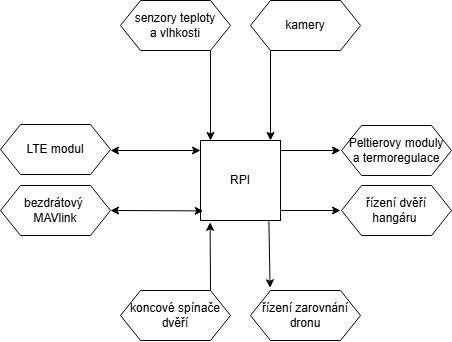
\includegraphics[width=0.75\linewidth]{schematics/Logic scheme.png}
            \caption{Schéma charakterizující vztahy řídící jednotky a ostatních modulů.}
        \end{figure}

    \subsection{Napájení} \label{subsec:napajeni}
        Napájanie celej „dokovacej stanice“ je možné rozdeliť na 3 hlavné časti. Každá z nich zabezpečuje čiastočne oddelenú funkciu, ktorá je nutná pre zabezpečenie stabilného napájania pre komponenty vo všetkých možných konfiguráciách hangáru.\\

        \noindent
        Hlavné napájanie hangáru zabezpečuje switching AC-DC zdroj, ktorý konvertuje štandardné napätie prenosovej sústavy, na 12V DC. Tento zdroj je umiestnený priamo v statickej časti dokovacej stanice a ku \acs{LP} je ďalej pripojený pomocou XT-60 konektorov. Konkrétny zdroj bol zvolený pre jeho prispôsobenosť na nepretržitú prevádzku a jeho dostupnosť, keďže je využívaný v množstve iných aplikácií. Je tiež dôležité spomenúť, že zdroj je od výroby utesnený pre ochranu proti vlhkosti a taktiež obsahuje prúdovú ochranu, ako aj ochranu proti prehriatiu. Konkrétne špecifikácie meničov je možné nájsť na stránkach predajcu \href{https://www.t-led.cz/p/led-zdroj-12v-600w-slim-12v-600w-56135}{tu}.\\

        \noindent
        Druhou súčasťou výkonovej elektroniky je zapojenie 2 DC-DC meničov, batérie a jej \uvoz{charge controllera}, ktoré je zobrazené na obrázku \ref{fig:el-gen-sch}.
        \begin{itemize}
            \item Oba DC-DC meniče slúžia na zvýšenie napätia poskytovaného zdrojom, resp. baterkou na napätia, ktoré sú nutné pre správne nabíjanie batérií v drone (Konverter č. 2-30V), ako aj nabíjanie záložných batérií priamo v dokovacej stanici (Konverter č. 1). Pridávajú taktiež flexibilitu v možnosti nastavenia nabíjacieho prúdu batérií. Ich použitie je potom dôležité aj z dôvodu meniaceho sa výstupného napätia batérie v dokovacej stanici, ktoré by mohlo obmedziť nabíjanie drona v prípade výpadku hlavného napájania. Konkrétne špecifikácie meničov je možné nájsť na stránkach predajcu \href{https://www.t-led.cz/p/led-zdroj-12v-600w-slim-12v-600w-56135}{tu}.
            
            \item Charge controller pre záložnú batériu zabezpečuje nabíjanie batérie, ako aj ochranu pred vybitím pod minimálne napätie. Umožňuje taktiež rýchlejšie a spoľahlivejšie spínanie napájania medzi batériou a hlavným zdrojom, ako by sme boli schopný jednoducho dosiahnuť diskrétnymi zapojením komponentov podľa vlastného návrhu. Rýchle spínanie je kritické pre mikropočítač \acs{RPI}, ktorý zabezpečuje riadenie a komunikáciu celého hangáru s okolím. Charge controller taktiež poskytuje možnosť nabíjania väčšieho množstva batérií naraz, čo je výhodné pre modulárnosť dokovacej stanice. Ovládanie všetkých záťaží je vykonávané \uvoz{LOAD} výstupom, ktorý je priamo pripojený k napájaniu \acs{RPI}, chladiacemu ventilátoru elektroniky a výstupnému relé. Zapojenie je zobrazené na obr \ref{fig:hp}.
        \end{itemize}

        \noindent
        Posledná časť, ktorá tvorí napájaciu časť elektroniky, sú relé, ktoré zabezpečujú prepnutie napájania medzi hlavným zdrojom a sadou záložných batérií a taktiež vypnutie väčšiny zariadení v dokovacej stanici v prípade, že dôjde k úplnému vybitiu záložných batérií.
        \begin{itemize}
            \item Zopnutie relé číslo 1 (obr \ref{fig:hp}) je ovládané hlavným zdrojom. Jeho úlohou je prepnutie napájania hangáru na záložný zdroj energie, v prípade výpadku hlavného napájania. Tak, ako je možné vidieť v schéme zapojenia, relé je pri normálnom fungovaní zopnuté, a teda hangár je napájaný z hlavného zdroja. Ak nastane výpadok elektrickej energie, dôjde k \uvoz{vypnutiu} relé. To má za následok pripojenie COM terminálu k záložnej batérii. Prepínanie relé číslo 1 mohlo byť zabezpečené aj mikropočítačom RPI, použité riešenie je však menej komplexné a preto sme ho zvolili.
            \item Relé číslo 2 má za úlohu odpojiť väčšinu elektroniky dokovacej stanice od napájania. Je ovládané priamo výstupom charge controllera batérie, odpojenie elektroniky je teda ovládané priamo ním a nastane v prípade, že dôjde k vybitiu záložnej batérie. 
        \end{itemize}

        \noindent
        Väčšina elektroniky dokovacej stanice je obsiahnutá v jednotnom oddelenom priestore, ktorý zabezpečuje jej adekvátne chladenie pomocou 2,80mm 12V ventilátorov.

        \begin{figure}[b]
            \centering
            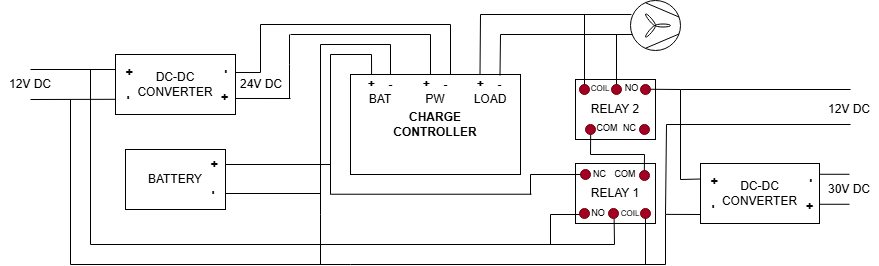
\includegraphics[width=1\linewidth]{schematics/HP module(3)_final.png}
            \caption{Schéma vysoko výkonnostní elektroniky.}
            \label{fig:hp}
        \end{figure}
    
    \subsection{Periferie}
    \label{subsec:periferie}
    Periferie hangáru slouží pro jeho interakci s okolím. Jedná se o následující části:
        \begin{enumerate}
            \item \hyperref[subsub:sht]{Senzory pro měření teploty}
            \item \hyperref[subsub:cams]{Kamery}
            \item \hyperref[subsub:stepmot]{Ovládání krokovacích motorů}
            \item \hyperref[subsub:dronmot]{Ovládání motorů zarovnávajících dron}
            \item \hyperref[subsub:pelt]{Peltierovy články pro termoregulaci}
            \item \hyperref[subsub:bat]{Modul pro odečítání stavu baterie}
        \end{enumerate}

    Dokumentace některých z těchto modulů se nachází na \href{https://github.com/BUT-DRONE-RESEARCH-CENTER/peripherals_hangar}{GitHub repozitáři periferií}.

    \begin{figure}[h!]
        \centering
        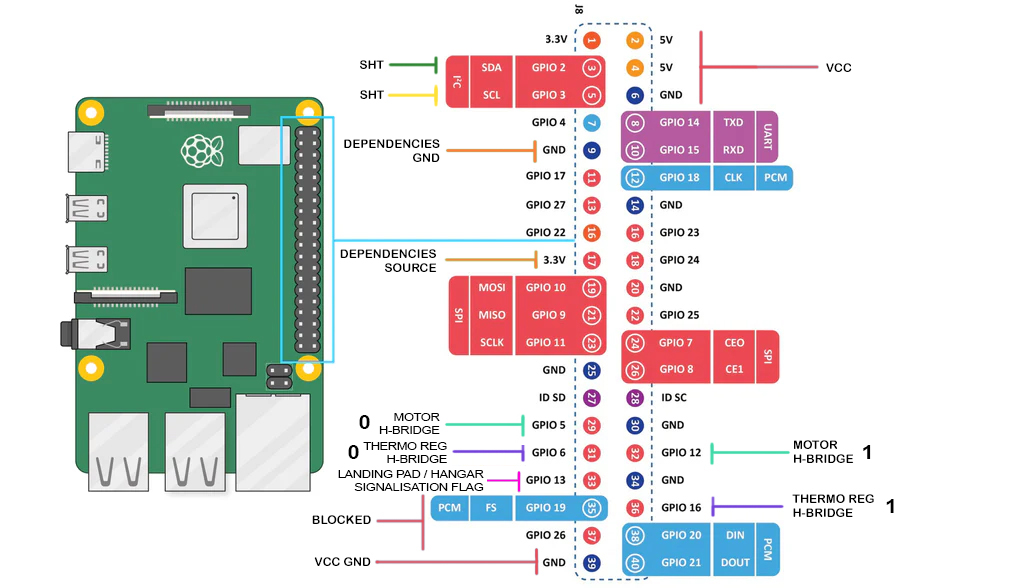
\includegraphics[width=1\linewidth]{schematics/GPIO_pinout.jpg}
        \caption{Zapojení GPIO pinů na jednodeskovém počítači \acs{RPI}.}
        \label{fig:GPIO}
    \end{figure}

    \subsubsection{Senzory pro měření teploty}
    \label{subsub:sht}
        Bylo použito dvou senzorů SHT. A to sice SHT-30 a SHT-25, kdy jeden senzor monitoruje vnitřní a druhý okolní teplotu hangáru. Komunikace s těmito senzory probíhá pomocí I$^2$C. Jednoduché programy v jazyce Python napsané pro sběr a zpracování dat o teplotě a vlhkosti data zpracovávají pomocí lineárních rovnic poskytnutých v dokumentaci modulu (např. pro \href{https://www.alldatasheet.com/datasheet-pdf/view/1522465/SENSIRION/SHT30-DIS.html}{SHT 30} v kapitole 4.14).\\
    
        \noindent
        Byť je sledování teploty žádoucí pouze v plné konfiguraci hangáru, je tento modul, v dosavadním stavu, přítomný přímo v \acs{LP} kvůli zjednodušení mechanické konstrukce.\\

    \subsubsection{Kamery}
    \label{subsub:cams}
        Pro pořízení obrazového záznamu v reálném čase je možné použít dva kamerové moduly, kdy jeden monitoruje stav uvnitř hangáru a druhý jeho okolí. Vybrané kamerové moduly jsou kompatibilní s knihovnou \textit{picamera2} v jazyce Python. Skript v jazyce Python napsaný pro ovládání těchto kamer navíc obsahuje jednoduchou, nastavitelnou logiku pro \uvoz{rotaci} pořízené záznamy tak, aby v případě neočekávané události mohl být její obrazový záznam zachován.\\
    
    \subsubsection{Ovládání krokových motorů}
    \label{subsub:stepmot}
        Krokové motory slouží k ovládání dveří hangáru. Samotným motorům se více věnuje kapitola \ref{sec:konstrukce}.\\
    
        \noindent
        Tato část je realizována za pomocí jednodeskového počítače \acs{UNO} s tzv. \uvoz{shieldem} pro ovládání CNC strojů (dále jen shield). Tento shield umožňuje pomocí ovladačů jednotlivých krokových motorů (těmi jsou diskrétní obvody). Komunikace s tímto shieldem probíhá sériovým portem COM mezi \acs{RPI} a \acs{UNO}. Na počítači \acs{UNO} je nahrán obraz open-source programu GBRL, který zpracovává příkazy v G-Code pro ovládání CNC strojů. Pomocí jednoduchých skriptů v jazyce Python jsou krokovým motorům posílány instrukce v jazyce G-Code. Takto jsou implementovány rutiny pro otevírání a zavírání dveří hangáru.
    
    \subsubsection{Ovládání motorů zarovnávajících dron}
    \label{subsub:dronmot}
        Těmito motory jsou GA12-N20 12V s převodovkou (více v kapitole \ref{sec:konstrukce}). Směr točení motorů je ovládán polaritou vstupního napětí. Standardně lze k těmto účelům využít tzv. \uvoz{H-Bridge}, neboli H-můstek integrovaný na jednom čipu. Kvůli nedostupnosti dostatečně výkonných modůlů H-Bridge, tak byl tento obvod nahrazen kombinací relé modulů, přesto může být na toto řešení v rámci dokumentace referováno jako na H-Bridge. Schéma použitého zapojení je na obrázku \ref{fig:hbridge}. Vstupem pro toto zapojení jsou logické signály \acs{RPI} z dvou výstupních GPIO pinů (viz obrázek \ref{fig:GPIO}, motor h-bridge).\\

        \begin{figure}[h!]
            \centering
            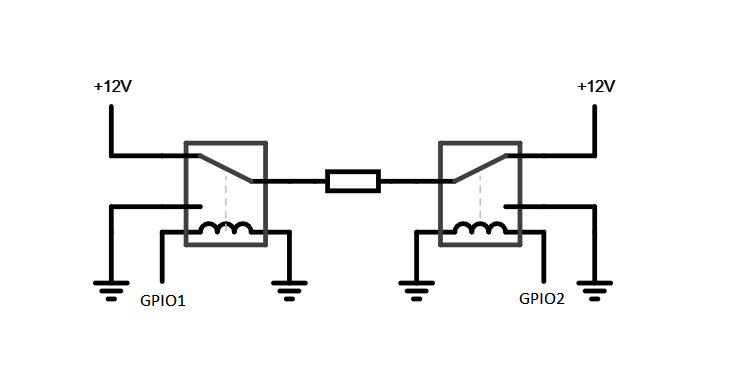
\includegraphics[width=0.75\linewidth]{schematics/circuit-20241208-1446.png}
            \caption{Náhradní zapojení pro \uvoz{H-Bridge} realizováno pomocí relé modulů.}
            \label{fig:hbridge}
        \end{figure}

        
    \subsubsection{Peltierovy články pro termoregulaci}
    \label{subsub:pelt}
        Obdobné jako v kapitole \ref{subsub:dronmot} je polarita teplotního rozdílu na obou stranách Peltierových modulů řízena polaritou přiloženého napětí. Proto se opět využívá H-Bridge modul. GPIO piny na počítači \acs{RPI} dedikované ovládání nastavení ohřevu, či ochlazování, jsou zobrazeny na obrázku \ref{fig:GPIO}.
    
    \subsubsection{Modul pro odečítání stavu baterie}
    \label{subsub:bat}
        Pro sledování napětí baterie byl použit jednoduchý napěťový dělič, který vytváří vhodný vstup pro modul s AD/DA převodníkem PCF8591. Tento modul pak odesílá data do \acs{RPI}, které je pomocí jednoduchého skriptu v jazyce Python zpracovává. Schéma tohoto zapojení je na obrázku \ref{fig:bat_readout}.

        \begin{figure}[h!]
            \centering
            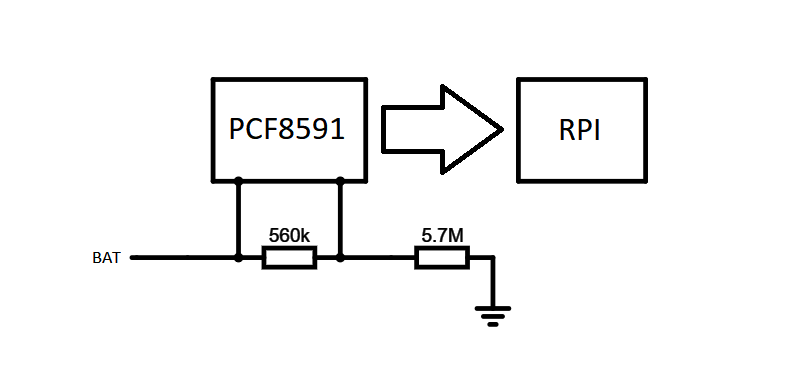
\includegraphics[width=0.75\linewidth]{schematics/BATcircuit-20241208-1501.png}
            \caption{Schéma pro modul sloužící pro sledování stavu baterie.}
            \label{fig:bat_readout}
        \end{figure}
        
\section{IT}  \label{sec:IT}
    \subsection{Softvérová architektúra hangáru}
    
    \subsection{Komunikace s dronem}
		Hangár zaisťuje samotú komunikáciu s dronom. Túto funkcionalitu zabezpečuje protokol MavLink, ktorý pomocou rádiovej komunikácie prenáša kritické dáta o stave dronu a zabezpečuje bezproblémovosť. Pripojenie na dron je zabezpečené vlastným python skriptom, vďaka ktorému vieme presne definovať informácie, ktoré sú dronom zasielané. Všetky dáta sa uschovávajú a potom preposielajú na server, kde si ich môže skontrolovať užívateľ. Pri strate spojenia (dron je mimo dosah) si program naďalej zabezpečuje informácie a do návratu drona. Protokol MavLink je doposiaľ nezávislý na hardvéry.    
    
    Softvérová architektúra hangáru pozostáva z dvoch hlavných častí: \textbf{vzdialeného servera} a \textbf{RPI skriptov}. Tieto komponenty spoločne zabezpečujú komplexné ovládanie a monitorovanie dronu a samotného hangáru.
    
    \subsubsection{Vzdialený server}
    Vzdialený server predstavuje webové rozhranie, ktoré umožňuje diaľkové ovládanie hangáru a dronu. Jeho najdôležitejšou úlohou je:
    \begin{itemize}
        \item spracovávanie dát prijímaných z RPI
        \item ich uchovávanie
        \item distribúcia pripojeným klientom
    \end{itemize}

    \noindent
    Jednou z hlavných výziev je nestabilná IP adresa RPI, ktorá sa mení v dôsledku využívania LTE modulu na pripojenie k internetu. Tento problém spôsobuje, že server musí pasívne čakať na prijatie prvého dátového paketu, aby si zaznamenal aktuálnu IP adresu odosielateľa. Ak sa IP adresa medzičasom zmení, môže dôjsť k zlyhaniu pri odosielaní príkazov.
    
    \subsubsection{Webové rozhranie}
    Webové rozhranie poskytuje rôzne užitočné informácie o stave dronu a hangáru. Obsahuje:
    \begin{itemize}
        \item živé video prenosy z troch kamier:
        \begin{itemize}
            \item jedna umiestnená na dronu
            \item dve monitorujúce interiér a okolie hangáru
        \end{itemize}
        \item mapu zobrazujúcu aktuálne polohy dronu a hangáru, vrátane informácií o ich vzájomnej vzdialenosti.
    \end{itemize}

    \noindent
    Medzi uchovávané údaje o dronu patria:
    \begin{itemize}[noitemsep, topsep=0pt]
        \item stav GPS
        \item pozícia
        \item rýchlosť
        \item dĺžka letu
        \item stav batérie
    \end{itemize}
    \vspace{.3cm}

    \noindent
    O stave hangáru sú dostupné nasledovné údaje:
    \begin{itemize}[noitemsep, topsep=0pt]
        \item teplota a vlhkosť
        \item stav nabíjania a napájania
        \item poloha dverí
        \item celkový stav hangáru
    \end{itemize}
    \vspace{.3cm}

    \noindent
    V sekcii nastavení je možné:
    \begin{itemize}[noitemsep, topsep=0pt]
        \item ovládať dvere
        \item nastavovať teplotu vnútorného vyhrievania
    \end{itemize}
    \vspace{.3cm}
    
    \noindent
    V pokročilej časti \texttt{s\_var} je umožnená úprava všetkých premenných skriptov bežiacich na RPI. Tento modul poskytuje takmer 100~\% prispôsobiteľnosť správania RPI. Typy premenných sú striktne kontrolované, pričom zmena hodnoty na hodnotu iného typu vyžaduje explicitné potvrdenie používateľom. Tento mechanizmus:
    \begin{enumerate}
        \item minimalizuje riziko zavedenia chýb do skriptov
        \item núti používateľa dôkladne zvážiť vykonané zmeny
    \end{enumerate}

    \subsubsection{Skripty na RPI}
    Skripty na RPI spravujú fungovanie celého hangáru. Časť ovláda periférie a motory, iná zasa komunikuje z dronom. Sú centrálne spúšťané hlavným programom. Rozdelením na menšie časti sme zaručili modularitu a odolnosť voči chybám zavedeným napríklad nesprávnym používaním \texttt{s\_var} editoru vo webovom rozhraní.

\section{Závěr}
    Projekt Inteligentní hangár představuje inovativní řešení pro efektivní správu, údržbu a provoz dronů v různých podmínkách, což umožňuje větší míru automatizace v této oblasti. Realizace zahrnovala komplexní návrh mechanické konstrukce, vývoj elektronických komponentů a implementaci softwarové architektury. Záměrem byla maximální modularita, flexibilita a spolehlivost zařízení.\\

    \noindent
    Návrh \textbf{mechanické konstrukce} (kapitola \ref{sec:konstrukce}) zahrnoval vytvoření robustní, ale modulární základny, jejíž klíčové komponenty zahrnují přistávací plochu (Landing Pad), zarovnávací mechanismus a dveře chránící dron před vnějšími vlivy. Design byl zvolen tak, aby byla zaručena pevnost, nízká hmotnost a snadná montáž.\\

    \noindent
    \textbf{Elektronická část} (kapitola \ref{sec:elektronika}) zahrnuje řídicí jednotku založenou na Raspberry Pi 5 a Arduino UNO, systémy napájení, senzory a periferie, jako jsou kamery a termoregulační prvky. Důraz byl kladen na automatické nabíjení dronů, monitorování prostředí, odolnost vůči vnějším vlivům a spolehlivost při výpadcích síťového napájení.\\

    \noindent
    \textbf{Softwarová architektura} (kapitola \ref{sec:IT}) poskytuje webové rozhraní umožňující vzdálené ovládání zařízení a komunikaci s dronem. Tato část projektu klade důraz na uživatelskou přívětivost a přizpůsobitelnost. Zabývá se zpracováním komunikace mezi hangárem a serverem. Poskytuje uživateli nastavitelné parametry pro provoz hangáru.\\

    \noindent
    Projekt nabízí široké spektrum aplikací. Především otevírá dveře nové generaci automatizace nákladných rutin dnes stále vykonávaných člověkem (monitoring špatně dostupných nebo nebezpečných oblastí, atp.). Součástí vývoje byla také popularizace projektu, která vyvolala kladnou odezvu. Můžeme tedy říct, že o takovouto technologii je na trhu zájem.
\newpage
\listoffigures

% tato sekce obsahuje prilohy
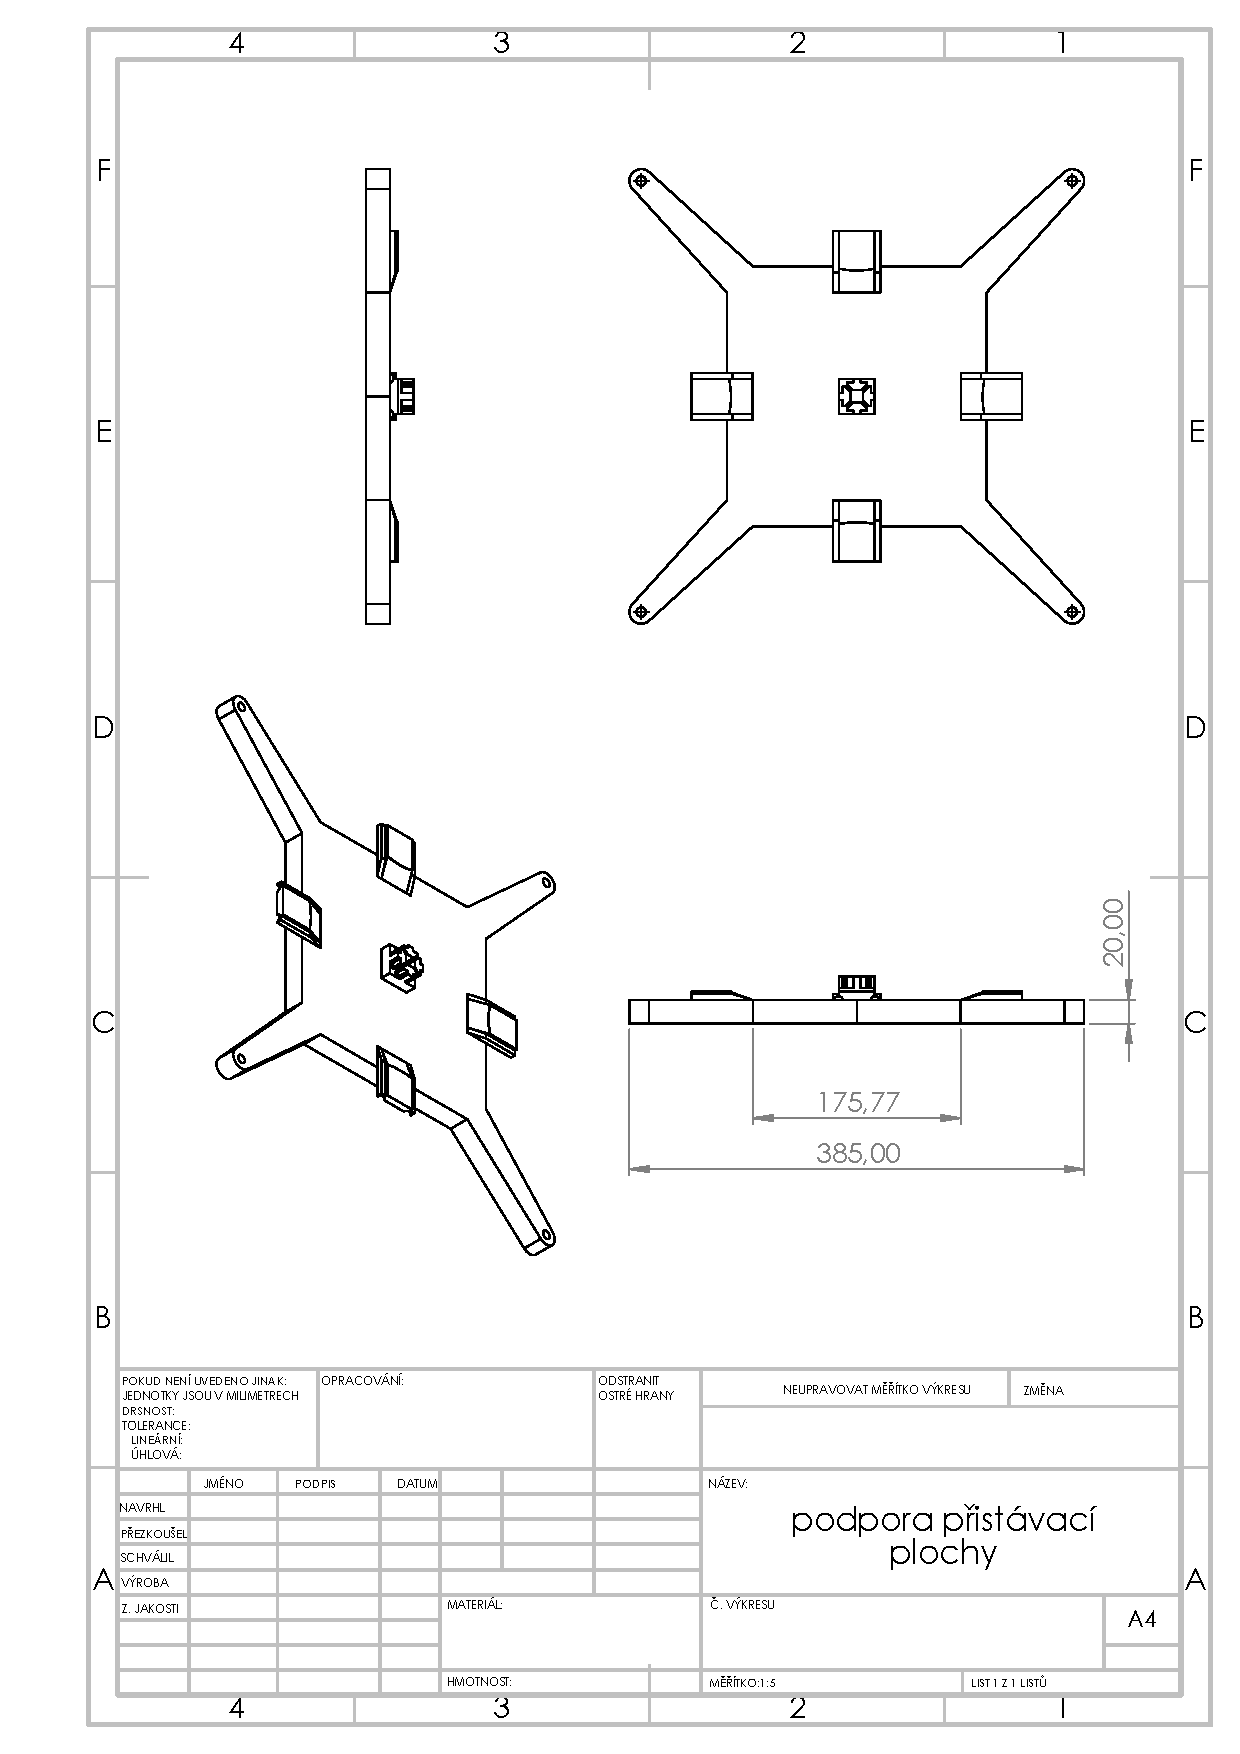
\includepdf[pages=-,addtotoc={1,section,1,Výkresy,mylabel}]{drawings/MODEL 1.pdf} \label{dwg:1}
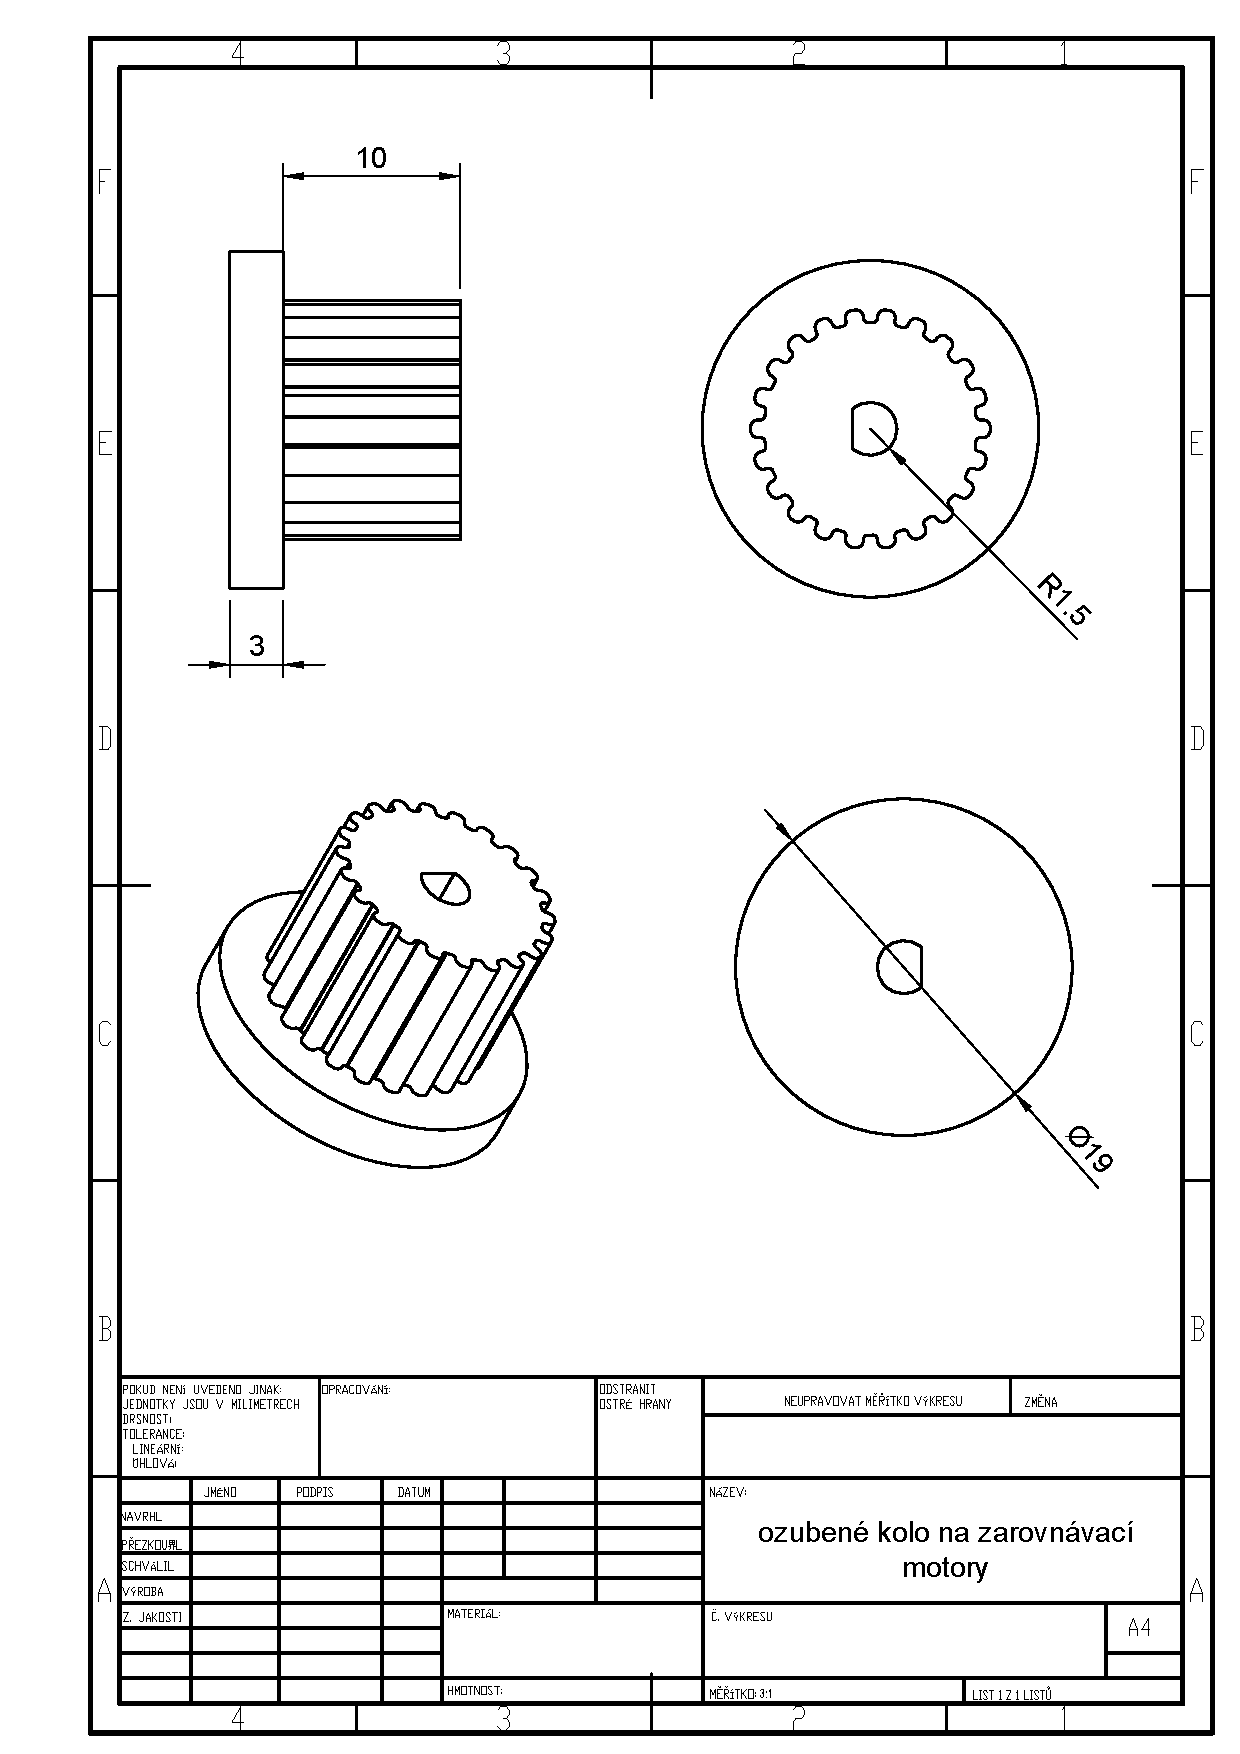
\includepdf{drawings/MODEL 2.pdf} \label{dwg:2}
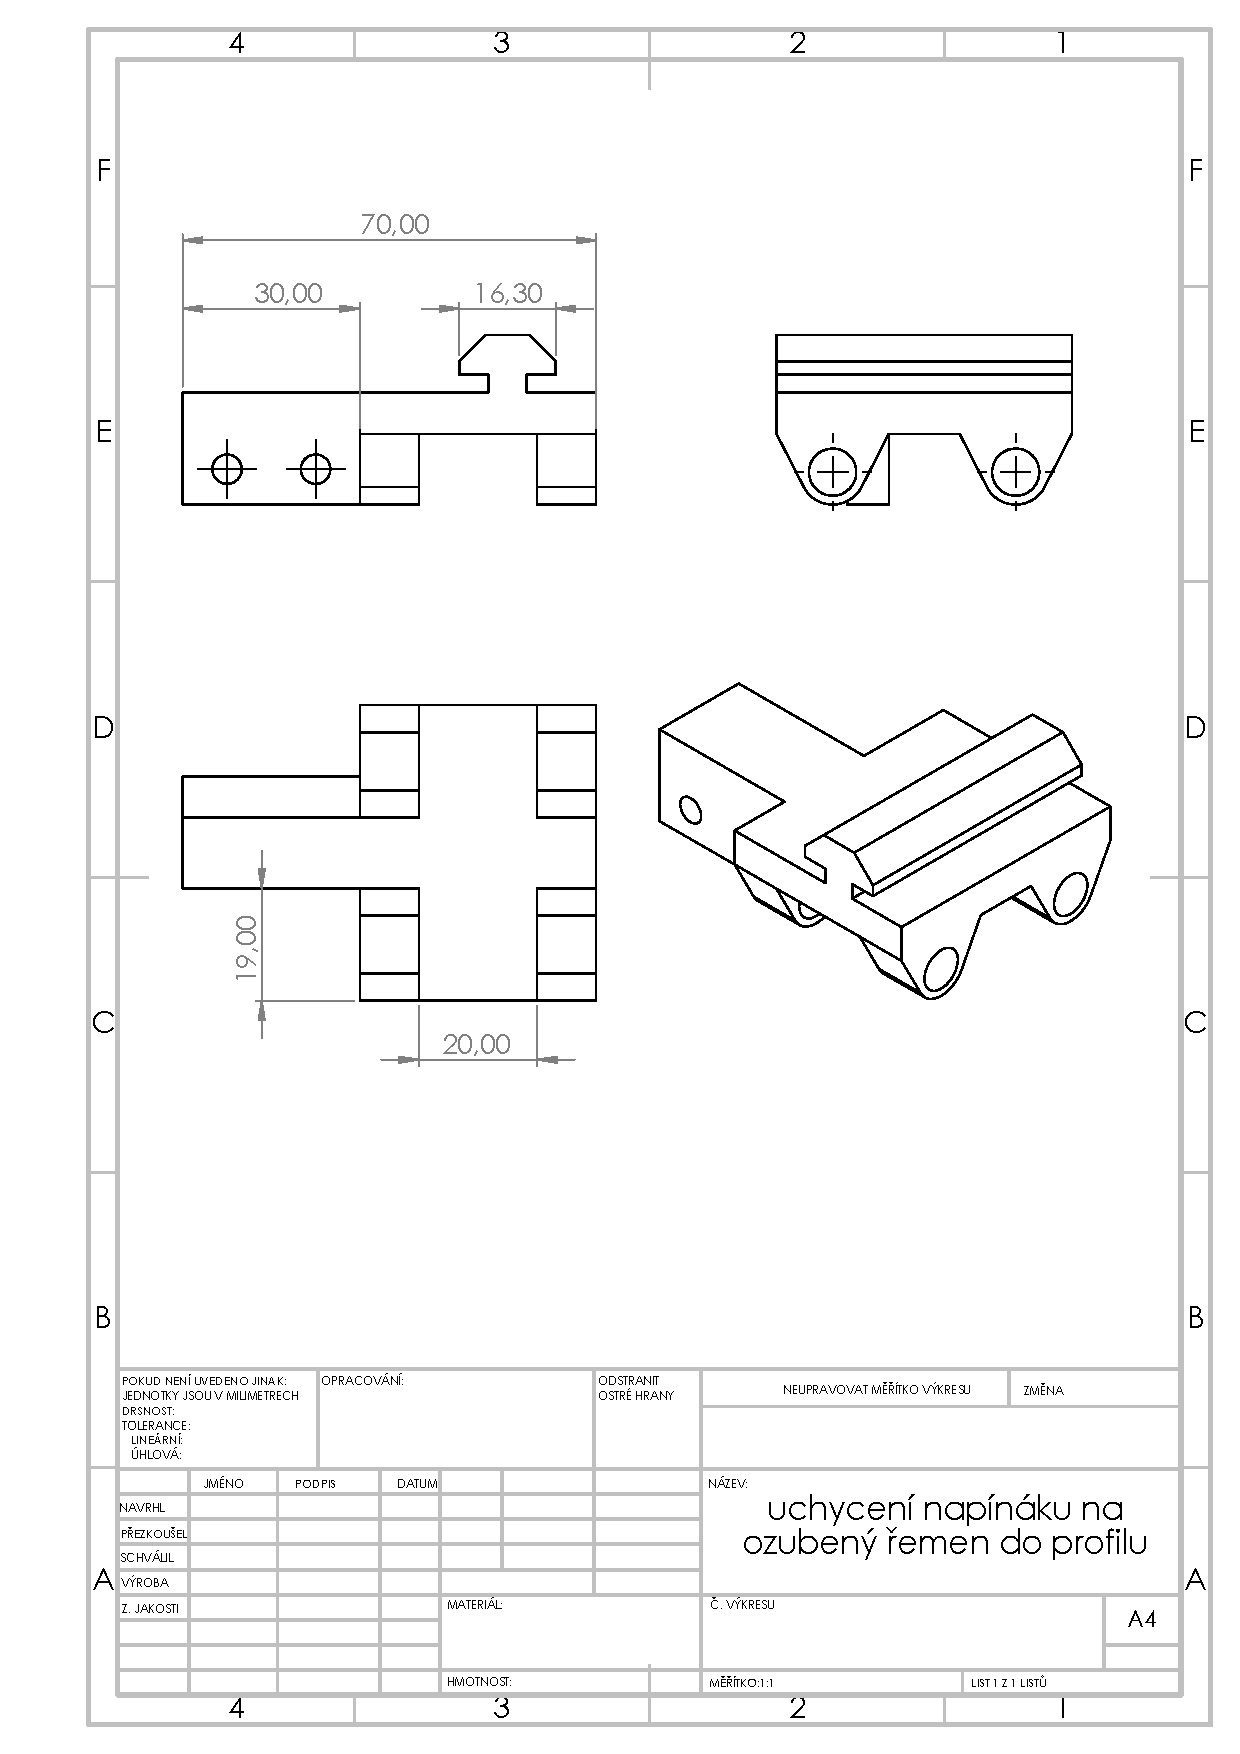
\includepdf{drawings/MODEL 3.pdf} \label{dwg:3}
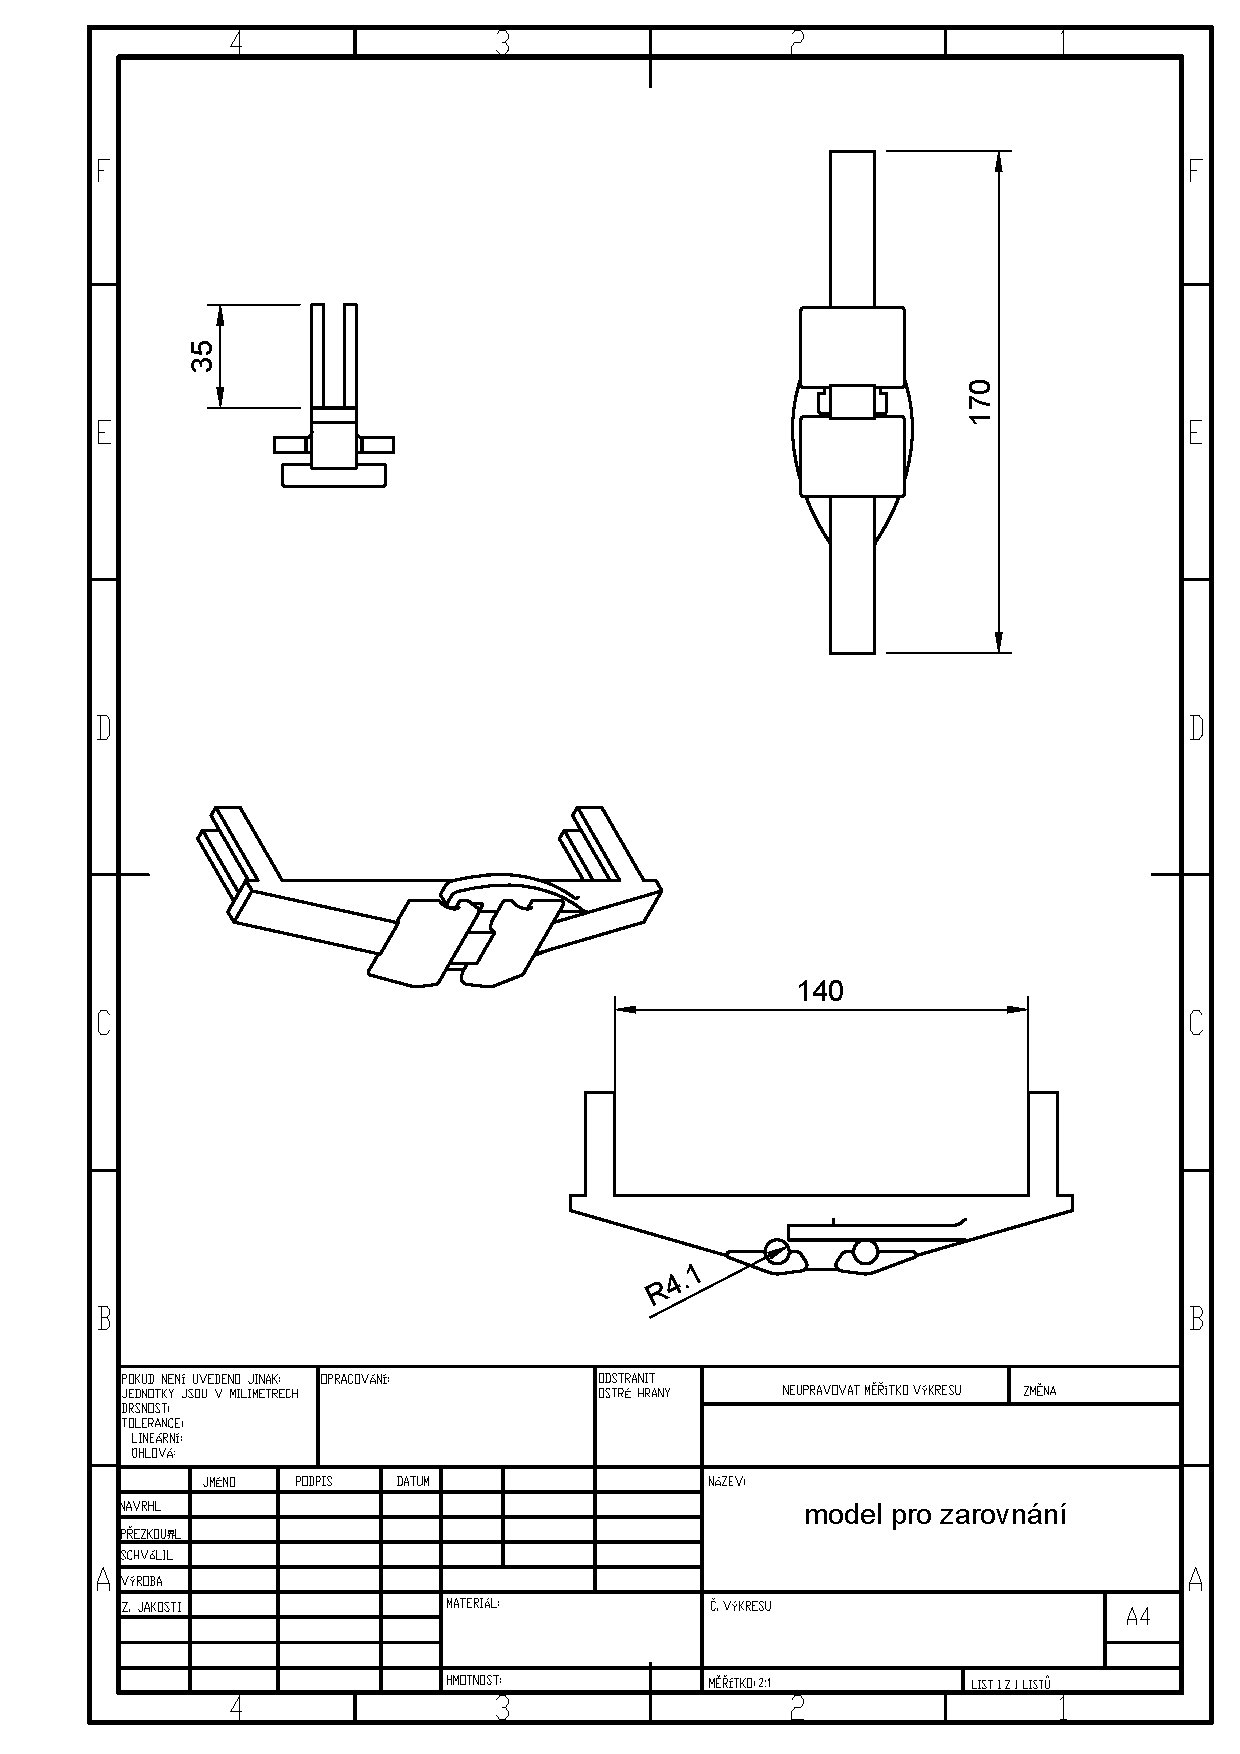
\includepdf{drawings/MODEL 4.pdf} \label{dwg:4}
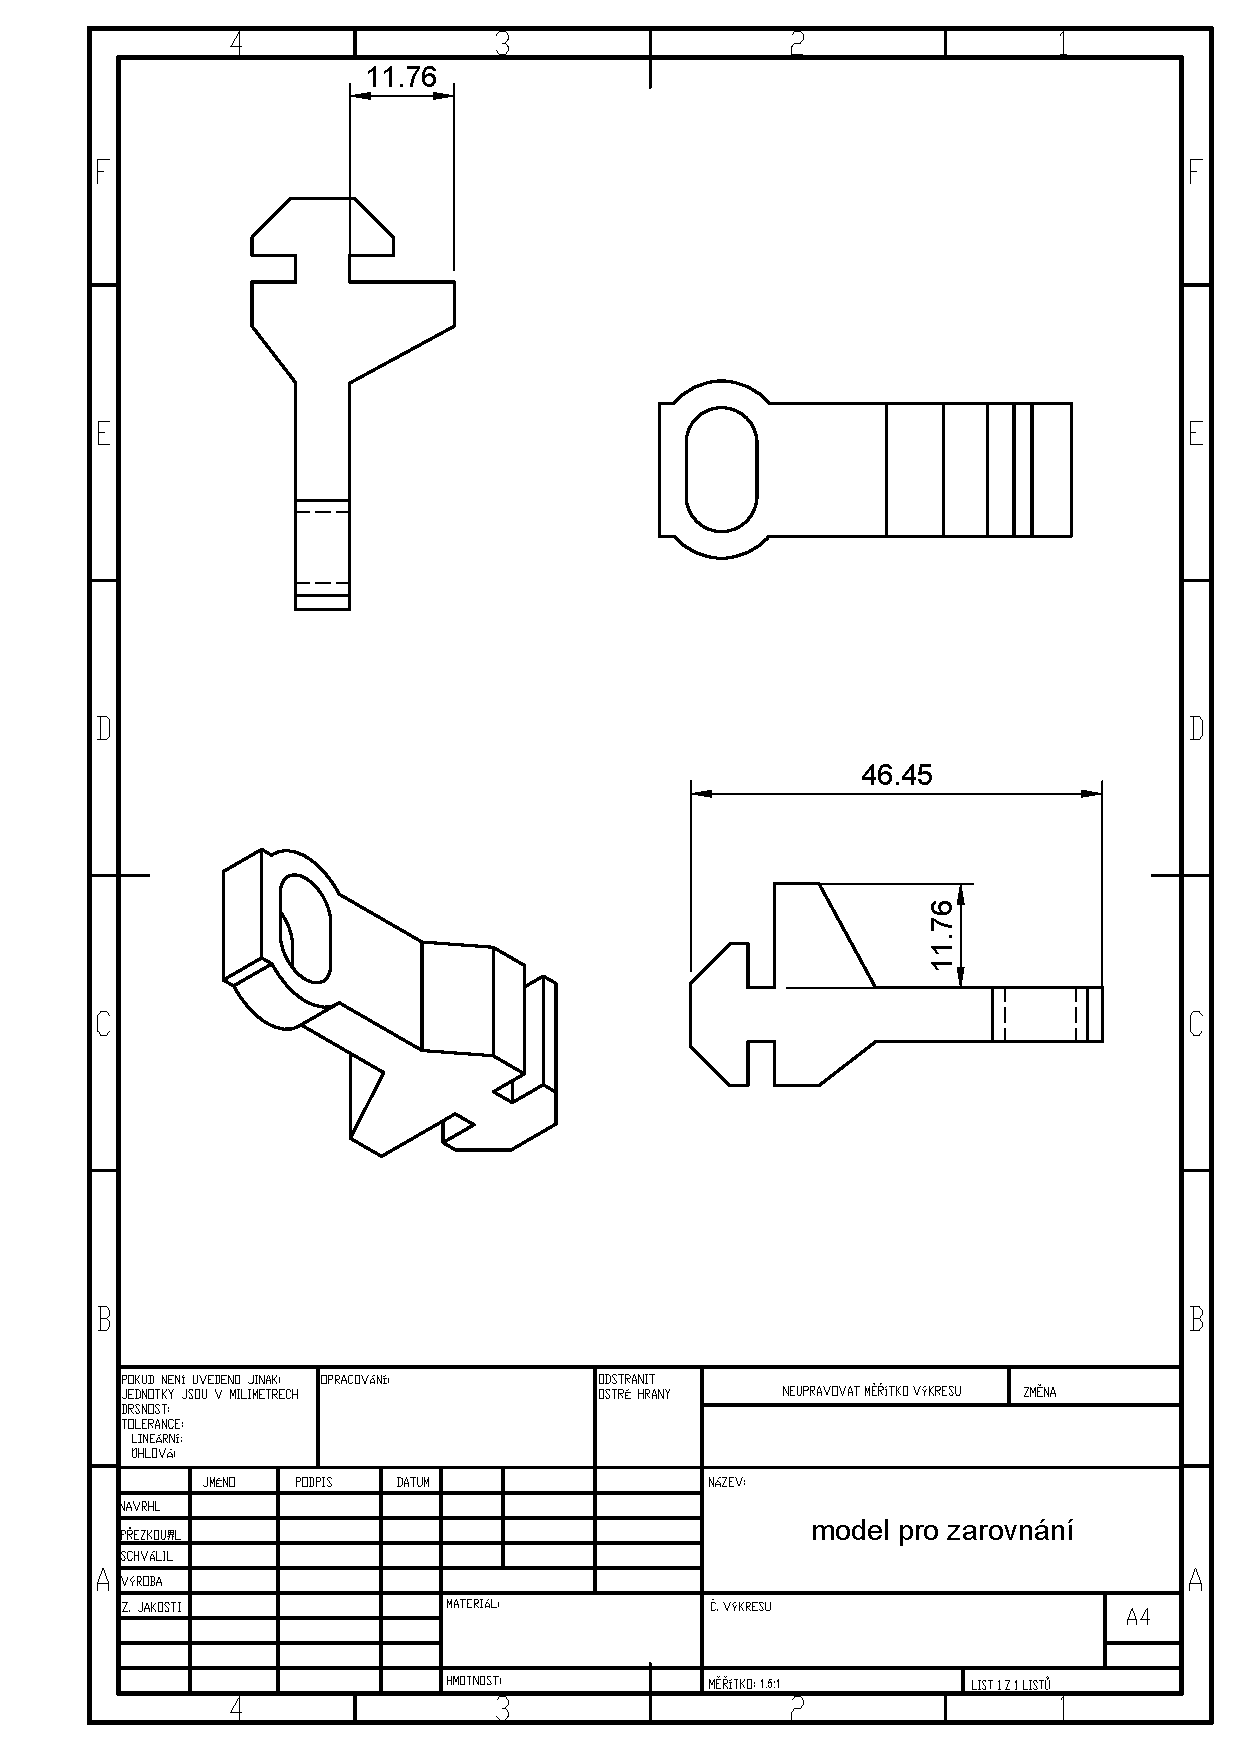
\includepdf{drawings/MODEL 5.pdf} \label{dwg:5}
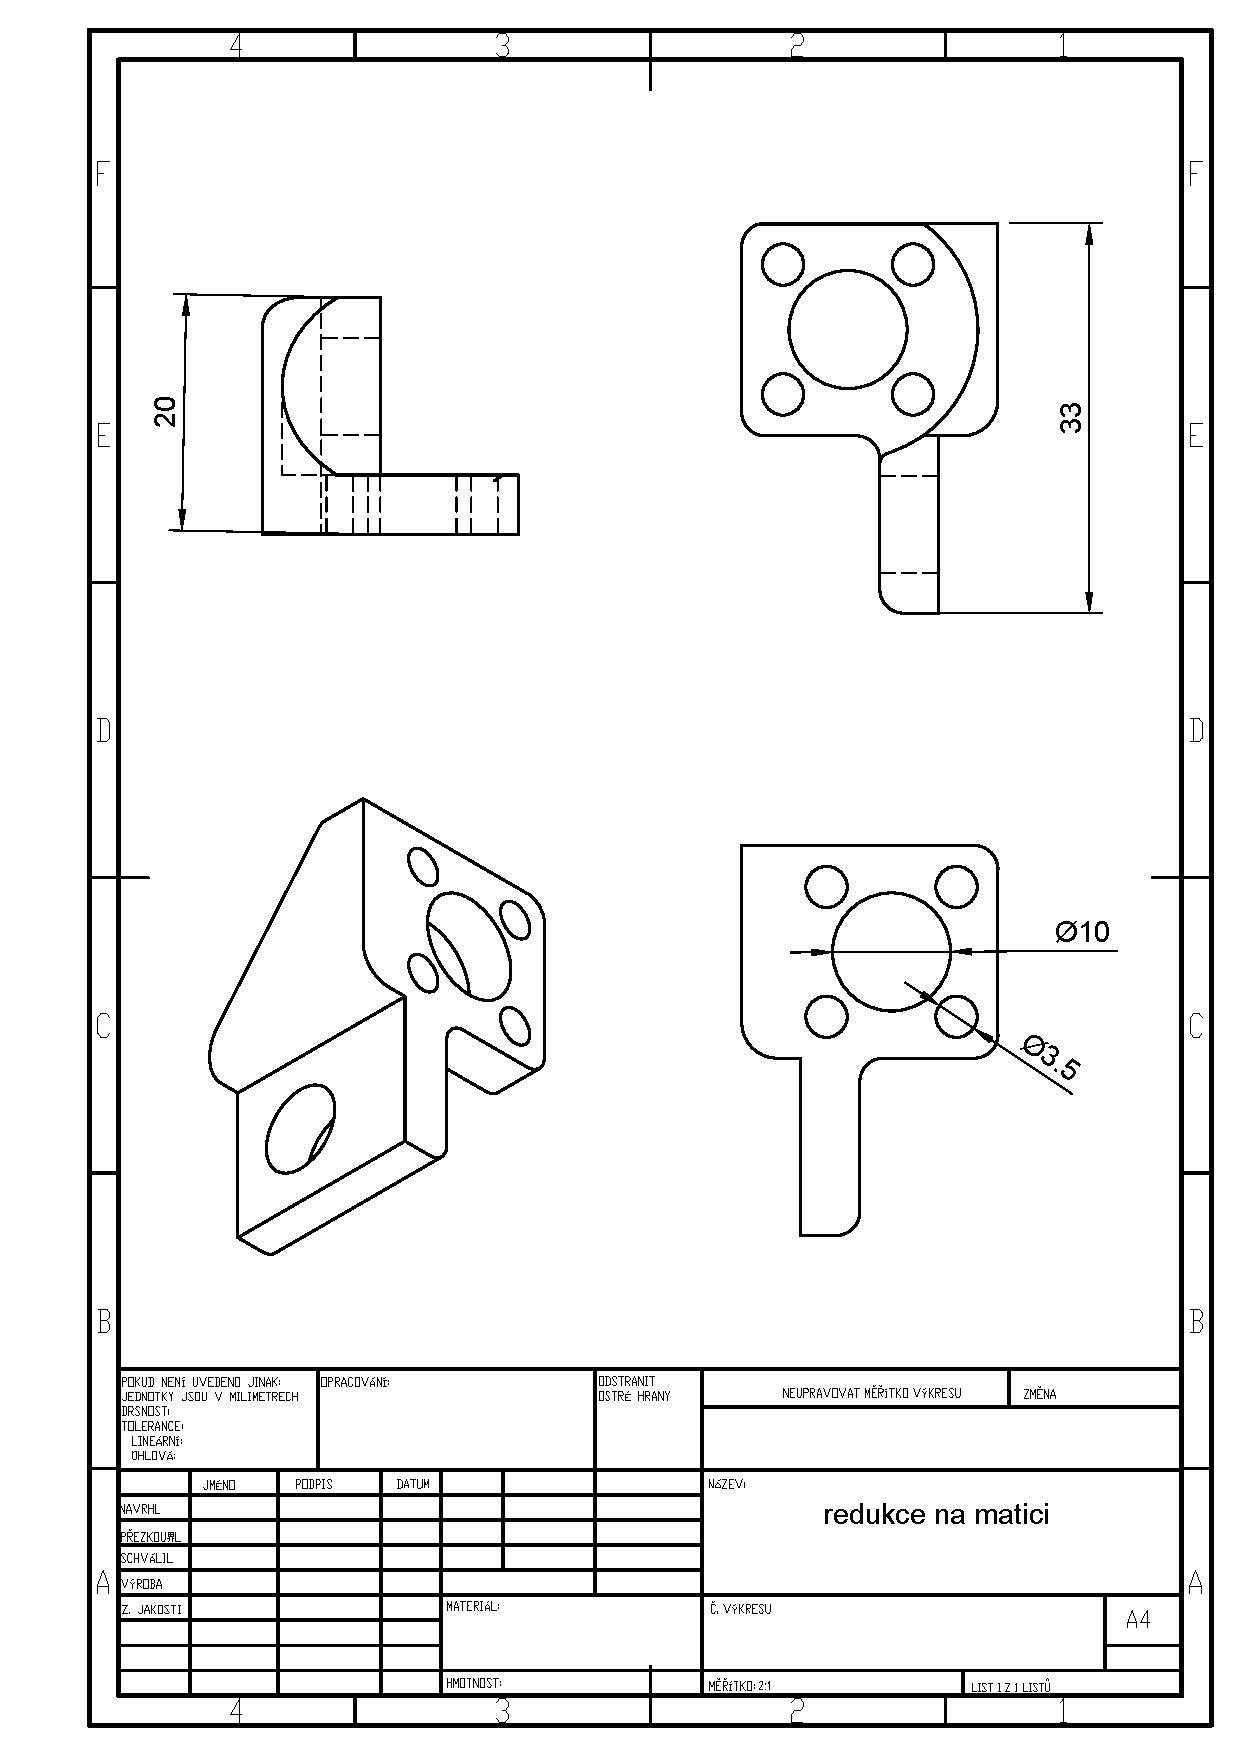
\includepdf{drawings/MODEL 6.pdf} \label{dwg:6}
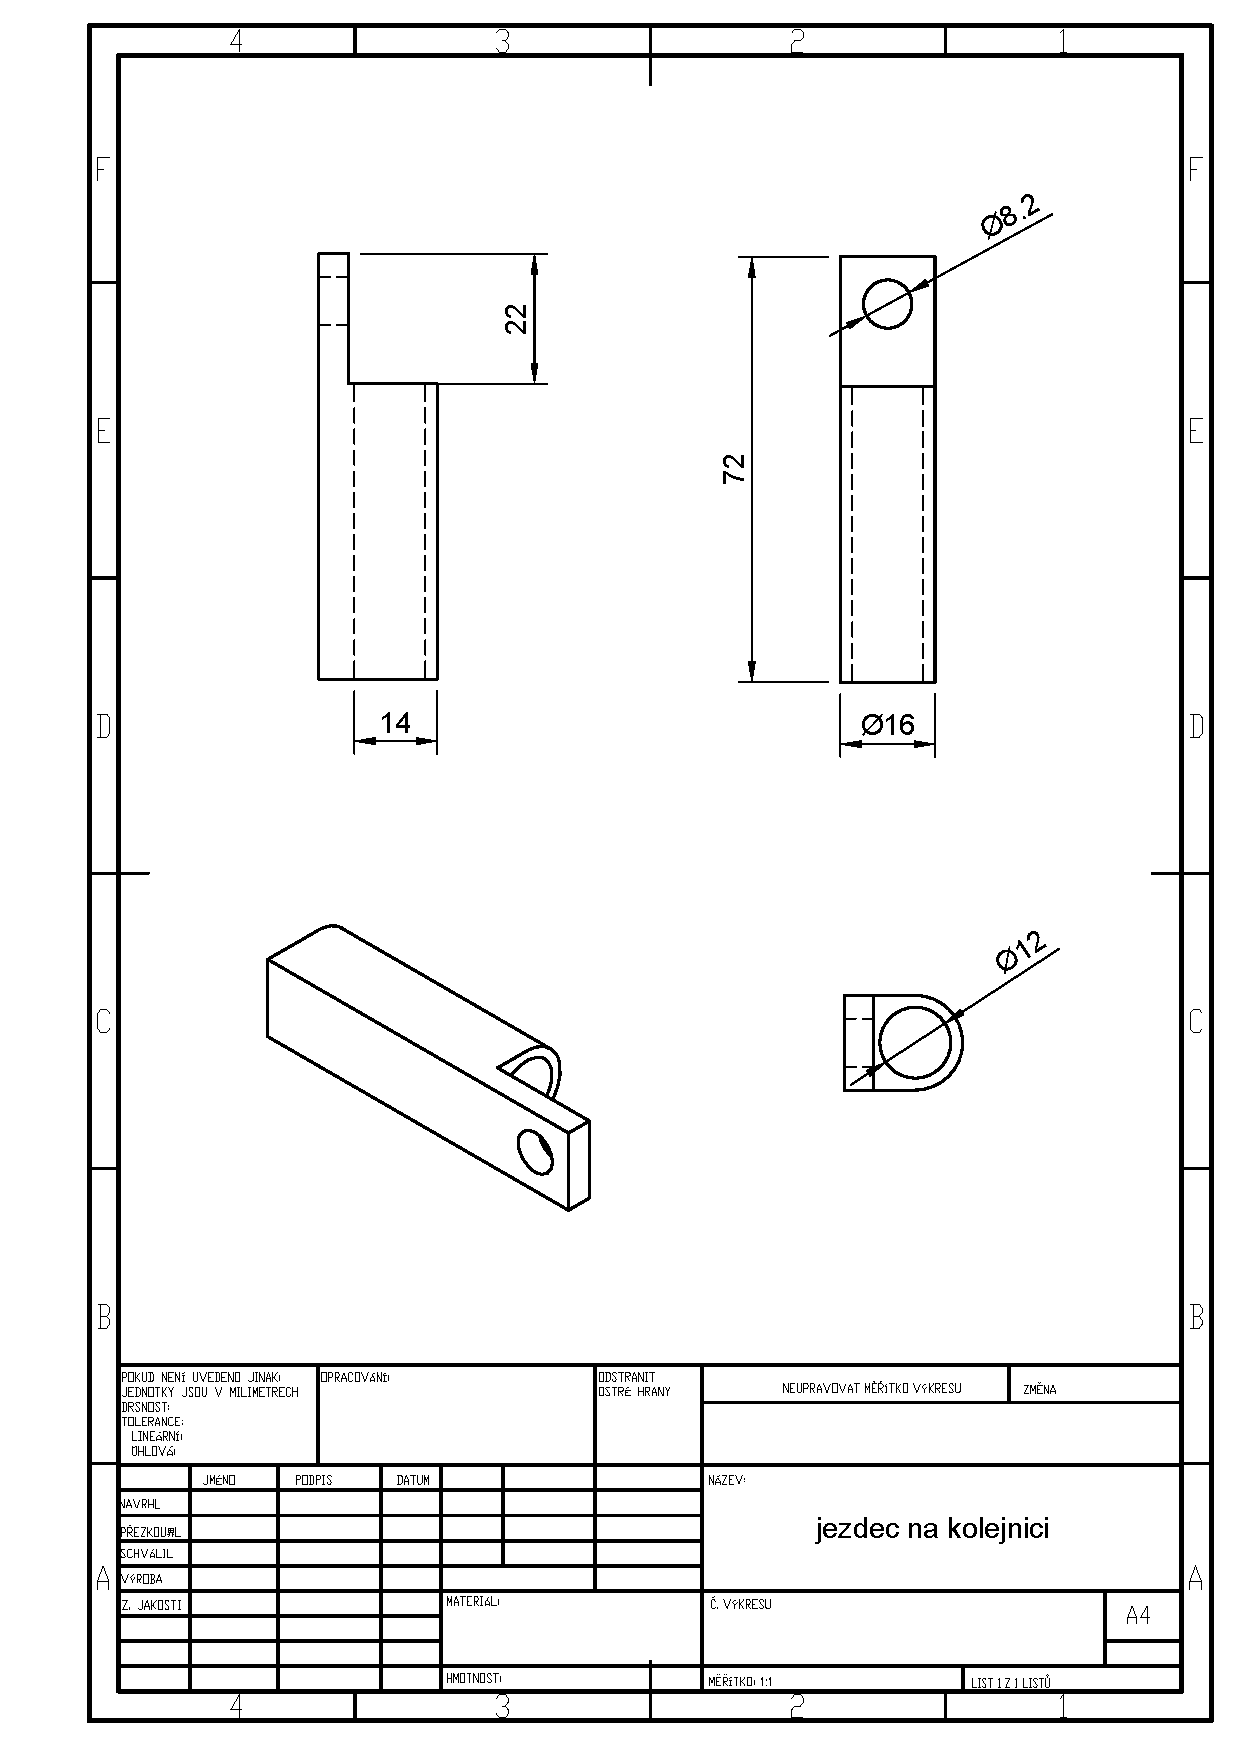
\includepdf{drawings/MODEL 7.pdf} \label{dwg:7}
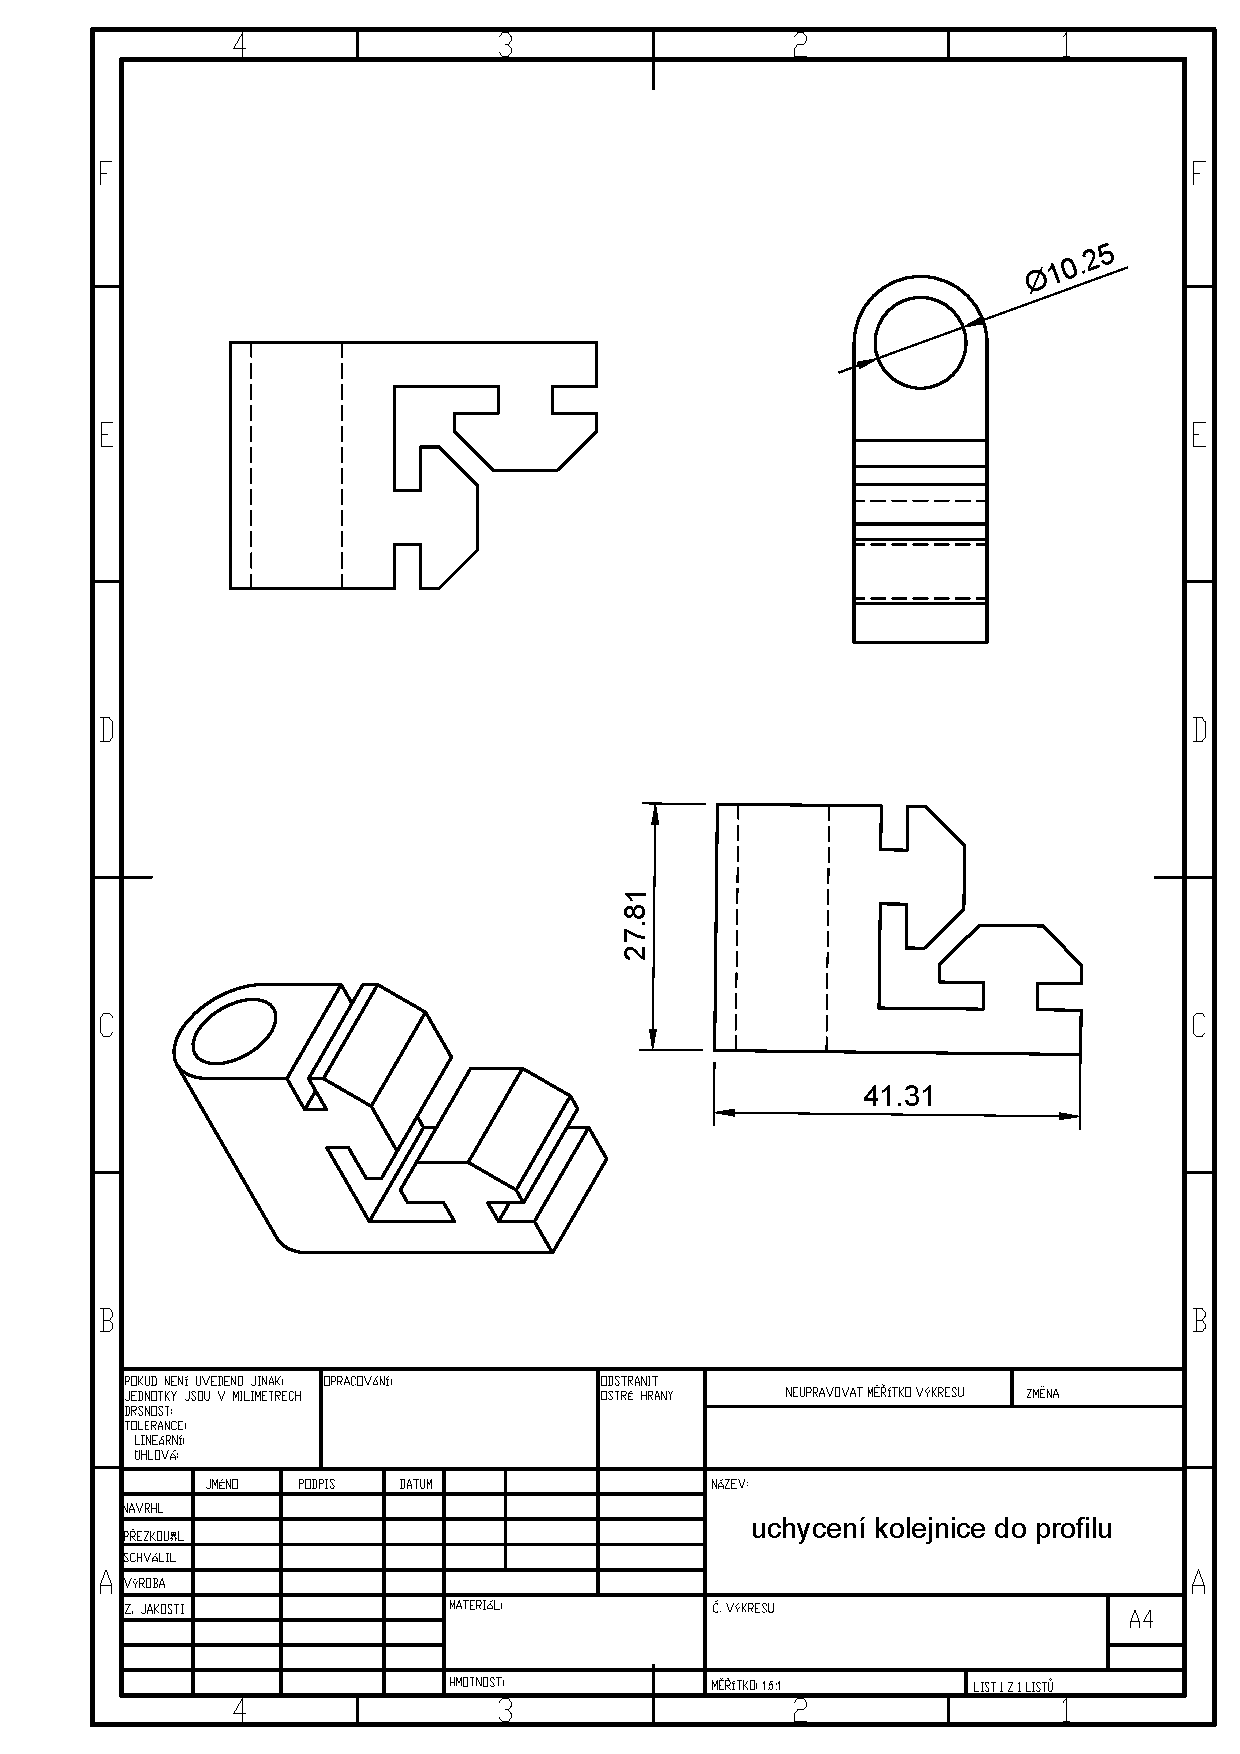
\includepdf{drawings/MODEL 8.pdf} \label{dwg:8}

\end{document}
